\documentclass[1p]{elsarticle_modified}
%\bibliographystyle{elsarticle-num}

%\usepackage[colorlinks]{hyperref}
%\usepackage{abbrmath_seonhwa} %\Abb, \Ascr, \Acal ,\Abf, \Afrak
\usepackage{amsfonts}
\usepackage{amssymb}
\usepackage{amsmath}
\usepackage{amsthm}
\usepackage{scalefnt}
\usepackage{amsbsy}
\usepackage{kotex}
\usepackage{caption}
\usepackage{subfig}
\usepackage{color}
\usepackage{graphicx}
\usepackage{xcolor} %% white, black, red, green, blue, cyan, magenta, yellow
\usepackage{float}
\usepackage{setspace}
\usepackage{hyperref}

\usepackage{tikz}
\usetikzlibrary{arrows}

\usepackage{multirow}
\usepackage{array} % fixed length table
\usepackage{hhline}

%%%%%%%%%%%%%%%%%%%%%
\makeatletter
\renewcommand*\env@matrix[1][\arraystretch]{%
	\edef\arraystretch{#1}%
	\hskip -\arraycolsep
	\let\@ifnextchar\new@ifnextchar
	\array{*\c@MaxMatrixCols c}}
\makeatother %https://tex.stackexchange.com/questions/14071/how-can-i-increase-the-line-spacing-in-a-matrix
%%%%%%%%%%%%%%%

\usepackage[normalem]{ulem}

\newcommand{\msout}[1]{\ifmmode\text{\sout{\ensuremath{#1}}}\else\sout{#1}\fi}
%SOURCE: \msout is \stkout macro in https://tex.stackexchange.com/questions/20609/strikeout-in-math-mode

\newcommand{\cancel}[1]{
	\ifmmode
	{\color{red}\msout{#1}}
	\else
	{\color{red}\sout{#1}}
	\fi
}

\newcommand{\add}[1]{
	{\color{blue}\uwave{#1}}
}

\newcommand{\replace}[2]{
	\ifmmode
	{\color{red}\msout{#1}}{\color{blue}\uwave{#2}}
	\else
	{\color{red}\sout{#1}}{\color{blue}\uwave{#2}}
	\fi
}

\newcommand{\Sol}{\mathcal{S}} %segment
\newcommand{\D}{D} %diagram
\newcommand{\A}{\mathcal{A}} %arc


%%%%%%%%%%%%%%%%%%%%%%%%%%%%%5 test

\def\sl{\operatorname{\textup{SL}}(2,\Cbb)}
\def\psl{\operatorname{\textup{PSL}}(2,\Cbb)}
\def\quan{\mkern 1mu \triangleright \mkern 1mu}

\theoremstyle{definition}
\newtheorem{thm}{Theorem}[section]
\newtheorem{prop}[thm]{Proposition}
\newtheorem{lem}[thm]{Lemma}
\newtheorem{ques}[thm]{Question}
\newtheorem{cor}[thm]{Corollary}
\newtheorem{defn}[thm]{Definition}
\newtheorem{exam}[thm]{Example}
\newtheorem{rmk}[thm]{Remark}
\newtheorem{alg}[thm]{Algorithm}

\newcommand{\I}{\sqrt{-1}}
\begin{document}

%\begin{frontmatter}
%
%\title{Boundary parabolic representations of knots up to 8 crossings}
%
%%% Group authors per affiliation:
%\author{Yunhi Cho} 
%\address{Department of Mathematics, University of Seoul, Seoul, Korea}
%\ead{yhcho@uos.ac.kr}
%
%
%\author{Seonhwa Kim} %\fnref{s_kim}}
%\address{Center for Geometry and Physics, Institute for Basic Science, Pohang, 37673, Korea}
%\ead{ryeona17@ibs.re.kr}
%
%\author{Hyuk Kim}
%\address{Department of Mathematical Sciences, Seoul National University, Seoul 08826, Korea}
%\ead{hyukkim@snu.ac.kr}
%
%\author{Seokbeom Yoon}
%\address{Department of Mathematical Sciences, Seoul National University, Seoul, 08826,  Korea}
%\ead{sbyoon15@snu.ac.kr}
%
%\begin{abstract}
%We find all boundary parabolic representation of knots up to 8 crossings.
%
%\end{abstract}
%\begin{keyword}
%    \MSC[2010] 57M25 
%\end{keyword}
%
%\end{frontmatter}

%\linenumbers
%\tableofcontents
%
\newcommand\colored[1]{\textcolor{white}{\rule[-0.35ex]{0.8em}{1.4ex}}\kern-0.8em\color{red} #1}%
%\newcommand\colored[1]{\textcolor{white}{ #1}\kern-2.17ex	\textcolor{white}{ #1}\kern-1.81ex	\textcolor{white}{ #1}\kern-2.15ex\color{red}#1	}

{\Large $\underline{12a_{0765}~(K12a_{0765})}$}

\setlength{\tabcolsep}{10pt}
\renewcommand{\arraystretch}{1.6}
\vspace{1cm}\begin{tabular}{m{100pt}>{\centering\arraybackslash}m{274pt}}
\multirow{5}{120pt}{
	\centering
	\includegraphics[width=112pt]{../../../GIT/diagram.site/Diagrams/png/1566_12a_0765.png}\\
\ \ \ A knot diagram\footnotemark}&
\allowdisplaybreaks
\textbf{Linearized knot diagam} \\
\cline{2-2}
 &
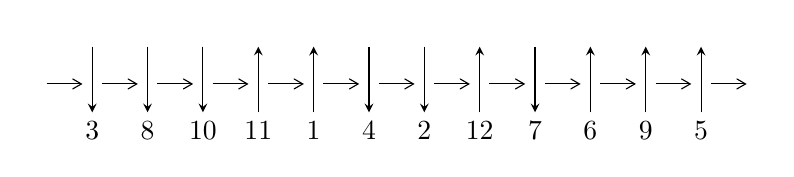
\begin{tikzpicture}[x=20pt, y=17pt]
	% nodes
	\node (C0) at (0, 0) {};
	\node (C1) at (1, 0) {};
	\node (C1U) at (1, +1) {};
	\node (C1D) at (1, -1) {3};

	\node (C2) at (2, 0) {};
	\node (C2U) at (2, +1) {};
	\node (C2D) at (2, -1) {8};

	\node (C3) at (3, 0) {};
	\node (C3U) at (3, +1) {};
	\node (C3D) at (3, -1) {10};

	\node (C4) at (4, 0) {};
	\node (C4U) at (4, +1) {};
	\node (C4D) at (4, -1) {11};

	\node (C5) at (5, 0) {};
	\node (C5U) at (5, +1) {};
	\node (C5D) at (5, -1) {1};

	\node (C6) at (6, 0) {};
	\node (C6U) at (6, +1) {};
	\node (C6D) at (6, -1) {4};

	\node (C7) at (7, 0) {};
	\node (C7U) at (7, +1) {};
	\node (C7D) at (7, -1) {2};

	\node (C8) at (8, 0) {};
	\node (C8U) at (8, +1) {};
	\node (C8D) at (8, -1) {12};

	\node (C9) at (9, 0) {};
	\node (C9U) at (9, +1) {};
	\node (C9D) at (9, -1) {7};

	\node (C10) at (10, 0) {};
	\node (C10U) at (10, +1) {};
	\node (C10D) at (10, -1) {6};

	\node (C11) at (11, 0) {};
	\node (C11U) at (11, +1) {};
	\node (C11D) at (11, -1) {9};

	\node (C12) at (12, 0) {};
	\node (C12U) at (12, +1) {};
	\node (C12D) at (12, -1) {5};
	\node (C13) at (13, 0) {};

	% arrows
	\draw[->,>={angle 60}]
	(C0) edge (C1) (C1) edge (C2) (C2) edge (C3) (C3) edge (C4) (C4) edge (C5) (C5) edge (C6) (C6) edge (C7) (C7) edge (C8) (C8) edge (C9) (C9) edge (C10) (C10) edge (C11) (C11) edge (C12) (C12) edge (C13) ;	\draw[->,>=stealth]
	(C1U) edge (C1D) (C2U) edge (C2D) (C3U) edge (C3D) (C4D) edge (C4U) (C5D) edge (C5U) (C6U) edge (C6D) (C7U) edge (C7D) (C8D) edge (C8U) (C9U) edge (C9D) (C10D) edge (C10U) (C11D) edge (C11U) (C12D) edge (C12U) ;
	\end{tikzpicture} \\
\hhline{~~} \\& 
\textbf{Solving Sequence} \\ \cline{2-2} 
 &
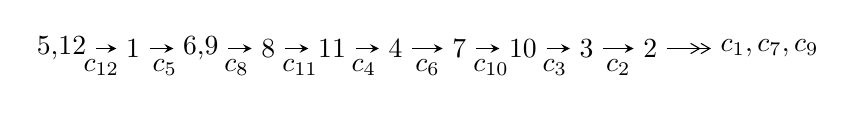
\begin{tikzpicture}[x=23pt, y=7pt]
	% node
	\node (A0) at (-1/8, 0) {5,12};
	\node (A1) at (1, 0) {1};
	\node (A2) at (33/16, 0) {6,9};
	\node (A3) at (25/8, 0) {8};
	\node (A4) at (33/8, 0) {11};
	\node (A5) at (41/8, 0) {4};
	\node (A6) at (49/8, 0) {7};
	\node (A7) at (57/8, 0) {10};
	\node (A8) at (65/8, 0) {3};
	\node (A9) at (73/8, 0) {2};
	\node (C1) at (1/2, -1) {$c_{12}$};
	\node (C2) at (3/2, -1) {$c_{5}$};
	\node (C3) at (21/8, -1) {$c_{8}$};
	\node (C4) at (29/8, -1) {$c_{11}$};
	\node (C5) at (37/8, -1) {$c_{4}$};
	\node (C6) at (45/8, -1) {$c_{6}$};
	\node (C7) at (53/8, -1) {$c_{10}$};
	\node (C8) at (61/8, -1) {$c_{3}$};
	\node (C9) at (69/8, -1) {$c_{2}$};
	\node (A10) at (11, 0) {$c_{1},c_{7},c_{9}$};

	% edge
	\draw[->,>=stealth]	
	(A0) edge (A1) (A1) edge (A2) (A2) edge (A3) (A3) edge (A4) (A4) edge (A5) (A5) edge (A6) (A6) edge (A7) (A7) edge (A8) (A8) edge (A9) ;
	\draw[->>,>={angle 60}]	
	(A9) edge (A10);
\end{tikzpicture} \\ 

\end{tabular} \\

\footnotetext{
The image of knot diagram is generated by the software ``\textbf{Draw programme}" developed by Andrew Bartholomew(\url{http://www.layer8.co.uk/maths/draw/index.htm\#Running-draw}), where we modified some parts for our purpose(\url{https://github.com/CATsTAILs/LinksPainter}).
}\phantom \\ \newline 
\centering \textbf{Ideals for irreducible components\footnotemark of $X_{\text{par}}$} 
 
\begin{align*}
I^u_{1}&=\langle 
6.98477\times10^{1451} u^{193}-1.16314\times10^{1452} u^{192}+\cdots+4.93072\times10^{1451} b+2.57314\times10^{1457},\\
\phantom{I^u_{1}}&\phantom{= \langle  }2.31622\times10^{1456} u^{193}-4.50288\times10^{1456} u^{192}+\cdots+1.21029\times10^{1457} a+5.08189\times10^{1461},\\
\phantom{I^u_{1}}&\phantom{= \langle  }u^{194}- u^{193}+\cdots-117893 u+245459\rangle \\
I^u_{2}&=\langle 
-1.19739\times10^{74} u^{55}+3.12250\times10^{74} u^{54}+\cdots+1.12058\times10^{71} b-1.63090\times10^{74},\\
\phantom{I^u_{2}}&\phantom{= \langle  }-1.86706\times10^{74} u^{55}+4.90830\times10^{74} u^{54}+\cdots+1.12058\times10^{71} a-2.71046\times10^{74},\;u^{56}-2 u^{55}+\cdots-2 u+1\rangle \\
\\
\end{align*}
\raggedright * 2 irreducible components of $\dim_{\mathbb{C}}=0$, with total 250 representations.\\
\footnotetext{All coefficients of polynomials are rational numbers. But the coefficients are sometimes approximated in decimal forms when there is not enough margin.}
\newpage
\renewcommand{\arraystretch}{1}
\centering \section*{I. $I^u_{1}= \langle 6.98\times10^{1451} u^{193}-1.16\times10^{1452} u^{192}+\cdots+4.93\times10^{1451} b+2.57\times10^{1457},\;2.32\times10^{1456} u^{193}-4.50\times10^{1456} u^{192}+\cdots+1.21\times10^{1457} a+5.08\times10^{1461},\;u^{194}- u^{193}+\cdots-117893 u+245459 \rangle$}
\flushleft \textbf{(i) Arc colorings}\\
\begin{tabular}{m{7pt} m{180pt} m{7pt} m{180pt} }
\flushright $a_{5}=$&$\begin{pmatrix}0\\u\end{pmatrix}$ \\
\flushright $a_{12}=$&$\begin{pmatrix}1\\0\end{pmatrix}$ \\
\flushright $a_{1}=$&$\begin{pmatrix}1\\- u^2\end{pmatrix}$ \\
\flushright $a_{6}=$&$\begin{pmatrix}u\\- u^3+u\end{pmatrix}$ \\
\flushright $a_{9}=$&$\begin{pmatrix}-0.191377 u^{193}+0.372050 u^{192}+\cdots+49992.0 u-41989.1\\-1.41658 u^{193}+2.35896 u^{192}+\cdots+1.03388\times10^{6} u-521859.\end{pmatrix}$ \\
\flushright $a_{8}=$&$\begin{pmatrix}1.22520 u^{193}-1.98691 u^{192}+\cdots-983885. u+479870.\\-1.41658 u^{193}+2.35896 u^{192}+\cdots+1.03388\times10^{6} u-521859.\end{pmatrix}$ \\
\flushright $a_{11}=$&$\begin{pmatrix}-4.07707 u^{193}+6.86053 u^{192}+\cdots+2.84866\times10^{6} u-1.46480\times10^{6}\\2.98731 u^{193}-5.04043 u^{192}+\cdots-2.05991\times10^{6} u+1.06527\times10^{6}\end{pmatrix}$ \\
\flushright $a_{4}=$&$\begin{pmatrix}3.93185 u^{193}-6.59426 u^{192}+\cdots-2.77115\times10^{6} u+1.42089\times10^{6}\\-2.17470 u^{193}+3.66893 u^{192}+\cdots+1.49760\times10^{6} u-775226.\end{pmatrix}$ \\
\flushright $a_{7}=$&$\begin{pmatrix}-7.14265 u^{193}+11.9908 u^{192}+\cdots+5.01907\times10^{6} u-2.57598\times10^{6}\\3.12899 u^{193}-5.27256 u^{192}+\cdots-2.17696\times10^{6} u+1.12123\times10^{6}\end{pmatrix}$ \\
\flushright $a_{10}=$&$\begin{pmatrix}-6.49999 u^{193}+10.9404 u^{192}+\cdots+4.53226\times10^{6} u-2.33266\times10^{6}\\1.69815 u^{193}-2.86783 u^{192}+\cdots-1.16638\times10^{6} u+604125.\end{pmatrix}$ \\
\flushright $a_{3}=$&$\begin{pmatrix}12.0920 u^{193}-20.3712 u^{192}+\cdots-8.40520\times10^{6} u+4.33186\times10^{6}\\-4.40681 u^{193}+7.44176 u^{192}+\cdots+3.03589\times10^{6} u-1.57018\times10^{6}\end{pmatrix}$ \\
\flushright $a_{2}=$&$\begin{pmatrix}7.98156 u^{193}-13.4540 u^{192}+\cdots-5.52815\times10^{6} u+2.85575\times10^{6}\\-2.41321 u^{193}+4.08087 u^{192}+\cdots+1.64843\times10^{6} u-856057.\end{pmatrix}$\\&\end{tabular}
\flushleft \textbf{(ii) Obstruction class $= -1$}\\~\\
\flushleft \textbf{(iii) Cusp Shapes $= -0.250556 u^{193}+0.556917 u^{192}+\cdots-23356.7 u-30204.0$}\\~\\
\newpage\renewcommand{\arraystretch}{1}
\flushleft \textbf{(iv) u-Polynomials at the component}\newline \\
\begin{tabular}{m{50pt}|m{274pt}}
Crossings & \hspace{64pt}u-Polynomials at each crossing \\
\hline $$\begin{aligned}c_{1}\end{aligned}$$&$\begin{aligned}
&u^{194}+93 u^{193}+\cdots+10148842326 u+242020249
\end{aligned}$\\
\hline $$\begin{aligned}c_{2},c_{7}\end{aligned}$$&$\begin{aligned}
&u^{194}+u^{193}+\cdots-18064 u+15557
\end{aligned}$\\
\hline $$\begin{aligned}c_{3}\end{aligned}$$&$\begin{aligned}
&u^{194}-2 u^{193}+\cdots-61 u+1
\end{aligned}$\\
\hline $$\begin{aligned}c_{4}\end{aligned}$$&$\begin{aligned}
&u^{194}-6 u^{192}+\cdots+43312357 u+11436607
\end{aligned}$\\
\hline $$\begin{aligned}c_{5},c_{12}\end{aligned}$$&$\begin{aligned}
&u^{194}+u^{193}+\cdots+117893 u+245459
\end{aligned}$\\
\hline $$\begin{aligned}c_{6}\end{aligned}$$&$\begin{aligned}
&u^{194}-11 u^{193}+\cdots-190 u+23
\end{aligned}$\\
\hline $$\begin{aligned}c_{8},c_{11}\end{aligned}$$&$\begin{aligned}
&u^{194}-15 u^{193}+\cdots+667643 u+215671
\end{aligned}$\\
\hline $$\begin{aligned}c_{9}\end{aligned}$$&$\begin{aligned}
&u^{194}-7 u^{193}+\cdots-76956 u+12989
\end{aligned}$\\
\hline $$\begin{aligned}c_{10}\end{aligned}$$&$\begin{aligned}
&u^{194}-3 u^{193}+\cdots+74 u+1
\end{aligned}$\\
\hline
\end{tabular}\\~\\
\newpage\renewcommand{\arraystretch}{1}
\flushleft \textbf{(v) Riley Polynomials at the component}\newline \\
\begin{tabular}{m{50pt}|m{274pt}}
Crossings & \hspace{64pt}Riley Polynomials at each crossing \\
\hline $$\begin{aligned}c_{1}\end{aligned}$$&$\begin{aligned}
&y^{194}+39 y^{193}+\cdots+4148575594390299166 y+58573800926022001
\end{aligned}$\\
\hline $$\begin{aligned}c_{2},c_{7}\end{aligned}$$&$\begin{aligned}
&y^{194}-93 y^{193}+\cdots-10148842326 y+242020249
\end{aligned}$\\
\hline $$\begin{aligned}c_{3}\end{aligned}$$&$\begin{aligned}
&y^{194}+4 y^{193}+\cdots+373 y+1
\end{aligned}$\\
\hline $$\begin{aligned}c_{4}\end{aligned}$$&$\begin{aligned}
&y^{194}-12 y^{193}+\cdots-567942991784177 y+130795979672449
\end{aligned}$\\
\hline $$\begin{aligned}c_{5},c_{12}\end{aligned}$$&$\begin{aligned}
&y^{194}-109 y^{193}+\cdots-3655898635621 y+60250120681
\end{aligned}$\\
\hline $$\begin{aligned}c_{6}\end{aligned}$$&$\begin{aligned}
&y^{194}-7 y^{193}+\cdots+26644 y+529
\end{aligned}$\\
\hline $$\begin{aligned}c_{8},c_{11}\end{aligned}$$&$\begin{aligned}
&y^{194}+93 y^{193}+\cdots+1846508165973 y+46513980241
\end{aligned}$\\
\hline $$\begin{aligned}c_{9}\end{aligned}$$&$\begin{aligned}
&y^{194}-9 y^{193}+\cdots+30908265410 y+168714121
\end{aligned}$\\
\hline $$\begin{aligned}c_{10}\end{aligned}$$&$\begin{aligned}
&y^{194}-15 y^{193}+\cdots-540 y+1
\end{aligned}$\\
\hline
\end{tabular}\\~\\
\newpage\flushleft \textbf{(vi) Complex Volumes and Cusp Shapes}
$$\begin{array}{c|c|c}  
\text{Solutions to }I^u_{1}& \I (\text{vol} + \sqrt{-1}CS) & \text{Cusp shape}\\
 \hline 
\begin{aligned}
u &= -0.406584 + 0.908345 I \\
a &= -0.73758 - 1.60254 I \\
b &= -0.353490 - 1.088290 I\end{aligned}
 & -6.07466 + 6.11744 I & \phantom{-0.000000 } 0 \\ \hline\begin{aligned}
u &= -0.406584 - 0.908345 I \\
a &= -0.73758 + 1.60254 I \\
b &= -0.353490 + 1.088290 I\end{aligned}
 & -6.07466 - 6.11744 I & \phantom{-0.000000 } 0 \\ \hline\begin{aligned}
u &= \phantom{-}0.926292 + 0.360172 I \\
a &= -0.364993 + 1.222190 I \\
b &= \phantom{-}0.003829 + 1.413000 I\end{aligned}
 & -1.86936 + 4.91916 I & \phantom{-0.000000 } 0 \\ \hline\begin{aligned}
u &= \phantom{-}0.926292 - 0.360172 I \\
a &= -0.364993 - 1.222190 I \\
b &= \phantom{-}0.003829 - 1.413000 I\end{aligned}
 & -1.86936 - 4.91916 I & \phantom{-0.000000 } 0 \\ \hline\begin{aligned}
u &= \phantom{-}0.676941 + 0.717325 I \\
a &= -0.49905 + 1.47156 I \\
b &= \phantom{-}0.815322 + 1.061790 I\end{aligned}
 & \phantom{-}0.25296 + 3.46087 I & \phantom{-0.000000 } 0 \\ \hline\begin{aligned}
u &= \phantom{-}0.676941 - 0.717325 I \\
a &= -0.49905 - 1.47156 I \\
b &= \phantom{-}0.815322 - 1.061790 I\end{aligned}
 & \phantom{-}0.25296 - 3.46087 I & \phantom{-0.000000 } 0 \\ \hline\begin{aligned}
u &= \phantom{-}0.979477 + 0.015977 I \\
a &= -1.25886 + 0.88498 I \\
b &= \phantom{-}0.706198 + 1.047070 I\end{aligned}
 & \phantom{-}3.24609 + 3.29684 I & \phantom{-0.000000 } 0 \\ \hline\begin{aligned}
u &= \phantom{-}0.979477 - 0.015977 I \\
a &= -1.25886 - 0.88498 I \\
b &= \phantom{-}0.706198 - 1.047070 I\end{aligned}
 & \phantom{-}3.24609 - 3.29684 I & \phantom{-0.000000 } 0 \\ \hline\begin{aligned}
u &= -0.554641 + 0.862200 I \\
a &= \phantom{-}0.070947 - 0.749012 I \\
b &= -0.415525 - 0.782291 I\end{aligned}
 & \phantom{-}0.300104 - 1.176760 I & \phantom{-0.000000 } 0 \\ \hline\begin{aligned}
u &= -0.554641 - 0.862200 I \\
a &= \phantom{-}0.070947 + 0.749012 I \\
b &= -0.415525 + 0.782291 I\end{aligned}
 & \phantom{-}0.300104 + 1.176760 I & \phantom{-0.000000 } 0\\
 \hline 
 \end{array}$$\newpage$$\begin{array}{c|c|c}  
\text{Solutions to }I^u_{1}& \I (\text{vol} + \sqrt{-1}CS) & \text{Cusp shape}\\
 \hline 
\begin{aligned}
u &= \phantom{-}0.417360 + 0.879928 I \\
a &= \phantom{-}0.87638 - 1.45101 I \\
b &= -0.055433 - 1.064100 I\end{aligned}
 & -3.55925 - 0.87375 I & \phantom{-0.000000 } 0 \\ \hline\begin{aligned}
u &= \phantom{-}0.417360 - 0.879928 I \\
a &= \phantom{-}0.87638 + 1.45101 I \\
b &= -0.055433 + 1.064100 I\end{aligned}
 & -3.55925 + 0.87375 I & \phantom{-0.000000 } 0 \\ \hline\begin{aligned}
u &= \phantom{-}0.694909 + 0.761600 I \\
a &= -0.069584 + 0.920006 I \\
b &= -0.081231 + 1.142800 I\end{aligned}
 & -3.53436 + 5.02332 I & \phantom{-0.000000 } 0 \\ \hline\begin{aligned}
u &= \phantom{-}0.694909 - 0.761600 I \\
a &= -0.069584 - 0.920006 I \\
b &= -0.081231 - 1.142800 I\end{aligned}
 & -3.53436 - 5.02332 I & \phantom{-0.000000 } 0 \\ \hline\begin{aligned}
u &= \phantom{-}0.906011 + 0.339014 I \\
a &= \phantom{-}1.48209 - 0.51804 I \\
b &= -0.807898 - 0.905467 I\end{aligned}
 & -3.12542 + 7.62172 I & \phantom{-0.000000 } 0 \\ \hline\begin{aligned}
u &= \phantom{-}0.906011 - 0.339014 I \\
a &= \phantom{-}1.48209 + 0.51804 I \\
b &= -0.807898 + 0.905467 I\end{aligned}
 & -3.12542 - 7.62172 I & \phantom{-0.000000 } 0 \\ \hline\begin{aligned}
u &= -0.920167 + 0.291516 I \\
a &= -0.026696 + 0.208084 I \\
b &= \phantom{-}1.006110 - 0.200811 I\end{aligned}
 & \phantom{-}1.71874 + 0.00266 I & \phantom{-0.000000 } 0 \\ \hline\begin{aligned}
u &= -0.920167 - 0.291516 I \\
a &= -0.026696 - 0.208084 I \\
b &= \phantom{-}1.006110 + 0.200811 I\end{aligned}
 & \phantom{-}1.71874 - 0.00266 I & \phantom{-0.000000 } 0 \\ \hline\begin{aligned}
u &= -1.006080 + 0.264880 I \\
a &= \phantom{-}1.336690 + 0.263964 I \\
b &= -0.601732 + 1.181270 I\end{aligned}
 & -4.18187 - 1.38142 I & \phantom{-0.000000 } 0 \\ \hline\begin{aligned}
u &= -1.006080 - 0.264880 I \\
a &= \phantom{-}1.336690 - 0.263964 I \\
b &= -0.601732 - 1.181270 I\end{aligned}
 & -4.18187 + 1.38142 I & \phantom{-0.000000 } 0\\
 \hline 
 \end{array}$$\newpage$$\begin{array}{c|c|c}  
\text{Solutions to }I^u_{1}& \I (\text{vol} + \sqrt{-1}CS) & \text{Cusp shape}\\
 \hline 
\begin{aligned}
u &= \phantom{-}0.569147 + 0.877802 I \\
a &= \phantom{-}0.09933 + 1.46827 I \\
b &= \phantom{-}0.341087 + 1.302340 I\end{aligned}
 & -4.05546 + 6.89533 I & \phantom{-0.000000 } 0 \\ \hline\begin{aligned}
u &= \phantom{-}0.569147 - 0.877802 I \\
a &= \phantom{-}0.09933 - 1.46827 I \\
b &= \phantom{-}0.341087 - 1.302340 I\end{aligned}
 & -4.05546 - 6.89533 I & \phantom{-0.000000 } 0 \\ \hline\begin{aligned}
u &= \phantom{-}0.672231 + 0.802747 I \\
a &= \phantom{-}1.00713 - 1.06155 I \\
b &= -0.004070 - 1.291130 I\end{aligned}
 & -3.52403 - 0.61398 I & \phantom{-0.000000 } 0 \\ \hline\begin{aligned}
u &= \phantom{-}0.672231 - 0.802747 I \\
a &= \phantom{-}1.00713 + 1.06155 I \\
b &= -0.004070 + 1.291130 I\end{aligned}
 & -3.52403 + 0.61398 I & \phantom{-0.000000 } 0 \\ \hline\begin{aligned}
u &= \phantom{-}0.505352 + 0.780497 I \\
a &= -0.73504 + 1.77591 I \\
b &= -0.061488 + 1.108370 I\end{aligned}
 & -7.58286 + 2.15592 I & \phantom{-0.000000 } 0 \\ \hline\begin{aligned}
u &= \phantom{-}0.505352 - 0.780497 I \\
a &= -0.73504 - 1.77591 I \\
b &= -0.061488 - 1.108370 I\end{aligned}
 & -7.58286 - 2.15592 I & \phantom{-0.000000 } 0 \\ \hline\begin{aligned}
u &= \phantom{-}0.888354 + 0.203742 I \\
a &= -2.91367 + 0.56000 I \\
b &= \phantom{-}0.224161 + 0.950037 I\end{aligned}
 & -6.60330 + 0.92815 I & \phantom{-0.000000 } 0 \\ \hline\begin{aligned}
u &= \phantom{-}0.888354 - 0.203742 I \\
a &= -2.91367 - 0.56000 I \\
b &= \phantom{-}0.224161 - 0.950037 I\end{aligned}
 & -6.60330 - 0.92815 I & \phantom{-0.000000 } 0 \\ \hline\begin{aligned}
u &= \phantom{-}0.050001 + 0.900877 I \\
a &= -0.061413 - 1.015520 I \\
b &= -0.802467 - 0.281089 I\end{aligned}
 & \phantom{-}1.87979 - 3.66071 I & \phantom{-0.000000 } 0 \\ \hline\begin{aligned}
u &= \phantom{-}0.050001 - 0.900877 I \\
a &= -0.061413 + 1.015520 I \\
b &= -0.802467 + 0.281089 I\end{aligned}
 & \phantom{-}1.87979 + 3.66071 I & \phantom{-0.000000 } 0\\
 \hline 
 \end{array}$$\newpage$$\begin{array}{c|c|c}  
\text{Solutions to }I^u_{1}& \I (\text{vol} + \sqrt{-1}CS) & \text{Cusp shape}\\
 \hline 
\begin{aligned}
u &= -0.713997 + 0.547809 I \\
a &= -0.438375 - 1.147880 I \\
b &= \phantom{-}0.08171 - 1.70026 I\end{aligned}
 & -5.00182 - 8.84965 I & \phantom{-0.000000 } 0 \\ \hline\begin{aligned}
u &= -0.713997 - 0.547809 I \\
a &= -0.438375 + 1.147880 I \\
b &= \phantom{-}0.08171 + 1.70026 I\end{aligned}
 & -5.00182 + 8.84965 I & \phantom{-0.000000 } 0 \\ \hline\begin{aligned}
u &= \phantom{-}0.820126 + 0.365115 I \\
a &= \phantom{-}0.82862 - 2.03229 I \\
b &= -0.042176 - 1.239600 I\end{aligned}
 & -6.33260 + 1.66013 I & \phantom{-0.000000 } 0 \\ \hline\begin{aligned}
u &= \phantom{-}0.820126 - 0.365115 I \\
a &= \phantom{-}0.82862 + 2.03229 I \\
b &= -0.042176 + 1.239600 I\end{aligned}
 & -6.33260 - 1.66013 I & \phantom{-0.000000 } 0 \\ \hline\begin{aligned}
u &= -1.106780 + 0.009307 I \\
a &= \phantom{-}0.448779 + 0.116546 I \\
b &= \phantom{-}0.538072 + 0.129745 I\end{aligned}
 & \phantom{-}2.61070 + 0.15227 I & \phantom{-0.000000 } 0 \\ \hline\begin{aligned}
u &= -1.106780 - 0.009307 I \\
a &= \phantom{-}0.448779 - 0.116546 I \\
b &= \phantom{-}0.538072 - 0.129745 I\end{aligned}
 & \phantom{-}2.61070 - 0.15227 I & \phantom{-0.000000 } 0 \\ \hline\begin{aligned}
u &= -0.874474 + 0.167435 I \\
a &= -1.64383 + 0.71858 I \\
b &= \phantom{-}0.647585 + 0.917707 I\end{aligned}
 & \phantom{-}1.27068 - 2.07977 I & \phantom{-0.000000 } 0 \\ \hline\begin{aligned}
u &= -0.874474 - 0.167435 I \\
a &= -1.64383 - 0.71858 I \\
b &= \phantom{-}0.647585 - 0.917707 I\end{aligned}
 & \phantom{-}1.27068 + 2.07977 I & \phantom{-0.000000 } 0 \\ \hline\begin{aligned}
u &= \phantom{-}0.868302 + 0.695008 I \\
a &= \phantom{-}0.017476 + 0.657665 I \\
b &= -0.588852 + 0.992156 I\end{aligned}
 & -3.10785 - 3.85382 I & \phantom{-0.000000 } 0 \\ \hline\begin{aligned}
u &= \phantom{-}0.868302 - 0.695008 I \\
a &= \phantom{-}0.017476 - 0.657665 I \\
b &= -0.588852 - 0.992156 I\end{aligned}
 & -3.10785 + 3.85382 I & \phantom{-0.000000 } 0\\
 \hline 
 \end{array}$$\newpage$$\begin{array}{c|c|c}  
\text{Solutions to }I^u_{1}& \I (\text{vol} + \sqrt{-1}CS) & \text{Cusp shape}\\
 \hline 
\begin{aligned}
u &= -0.251943 + 0.846329 I \\
a &= \phantom{-}0.170361 + 1.201550 I \\
b &= -0.925435 + 0.105369 I\end{aligned}
 & \phantom{-}0.58405 + 8.87272 I & \phantom{-0.000000 } 0 \\ \hline\begin{aligned}
u &= -0.251943 - 0.846329 I \\
a &= \phantom{-}0.170361 - 1.201550 I \\
b &= -0.925435 - 0.105369 I\end{aligned}
 & \phantom{-}0.58405 - 8.87272 I & \phantom{-0.000000 } 0 \\ \hline\begin{aligned}
u &= -1.089310 + 0.254934 I \\
a &= -2.04511 - 0.03490 I \\
b &= \phantom{-}0.425038 - 1.079870 I\end{aligned}
 & \phantom{-}0.63001 - 4.71909 I & \phantom{-0.000000 } 0 \\ \hline\begin{aligned}
u &= -1.089310 - 0.254934 I \\
a &= -2.04511 + 0.03490 I \\
b &= \phantom{-}0.425038 + 1.079870 I\end{aligned}
 & \phantom{-}0.63001 + 4.71909 I & \phantom{-0.000000 } 0 \\ \hline\begin{aligned}
u &= -0.493210 + 1.004910 I \\
a &= \phantom{-}0.72931 + 1.41815 I \\
b &= -0.601959 + 0.895829 I\end{aligned}
 & -0.09608 - 5.52301 I & \phantom{-0.000000 } 0 \\ \hline\begin{aligned}
u &= -0.493210 - 1.004910 I \\
a &= \phantom{-}0.72931 - 1.41815 I \\
b &= -0.601959 - 0.895829 I\end{aligned}
 & -0.09608 + 5.52301 I & \phantom{-0.000000 } 0 \\ \hline\begin{aligned}
u &= -0.958228 + 0.582368 I \\
a &= -0.56780 - 1.84248 I \\
b &= \phantom{-}0.571867 - 0.582135 I\end{aligned}
 & \phantom{-}3.64674 - 2.41351 I & \phantom{-0.000000 } 0 \\ \hline\begin{aligned}
u &= -0.958228 - 0.582368 I \\
a &= -0.56780 + 1.84248 I \\
b &= \phantom{-}0.571867 + 0.582135 I\end{aligned}
 & \phantom{-}3.64674 + 2.41351 I & \phantom{-0.000000 } 0 \\ \hline\begin{aligned}
u &= \phantom{-}0.742812 + 0.850574 I \\
a &= \phantom{-}0.98027 - 1.03175 I \\
b &= \phantom{-}0.001951 - 1.079380 I\end{aligned}
 & -3.66789 - 0.69831 I & \phantom{-0.000000 } 0 \\ \hline\begin{aligned}
u &= \phantom{-}0.742812 - 0.850574 I \\
a &= \phantom{-}0.98027 + 1.03175 I \\
b &= \phantom{-}0.001951 + 1.079380 I\end{aligned}
 & -3.66789 + 0.69831 I & \phantom{-0.000000 } 0\\
 \hline 
 \end{array}$$\newpage$$\begin{array}{c|c|c}  
\text{Solutions to }I^u_{1}& \I (\text{vol} + \sqrt{-1}CS) & \text{Cusp shape}\\
 \hline 
\begin{aligned}
u &= \phantom{-}1.054170 + 0.406779 I \\
a &= -0.224180 + 0.623710 I \\
b &= \phantom{-}1.40827 - 0.46099 I\end{aligned}
 & \phantom{-}4.63126 + 3.86923 I & \phantom{-0.000000 } 0 \\ \hline\begin{aligned}
u &= \phantom{-}1.054170 - 0.406779 I \\
a &= -0.224180 - 0.623710 I \\
b &= \phantom{-}1.40827 + 0.46099 I\end{aligned}
 & \phantom{-}4.63126 - 3.86923 I & \phantom{-0.000000 } 0 \\ \hline\begin{aligned}
u &= -1.051590 + 0.426304 I \\
a &= \phantom{-}1.52955 + 0.46597 I \\
b &= \phantom{-}0.114719 + 0.708966 I\end{aligned}
 & \phantom{-}1.29199 - 0.63572 I & \phantom{-0.000000 } 0 \\ \hline\begin{aligned}
u &= -1.051590 - 0.426304 I \\
a &= \phantom{-}1.52955 - 0.46597 I \\
b &= \phantom{-}0.114719 - 0.708966 I\end{aligned}
 & \phantom{-}1.29199 + 0.63572 I & \phantom{-0.000000 } 0 \\ \hline\begin{aligned}
u &= -1.113500 + 0.254079 I \\
a &= -0.388065 + 0.108602 I \\
b &= \phantom{-}1.38923 + 0.48796 I\end{aligned}
 & \phantom{-}4.40392 - 3.71450 I & \phantom{-0.000000 } 0 \\ \hline\begin{aligned}
u &= -1.113500 - 0.254079 I \\
a &= -0.388065 - 0.108602 I \\
b &= \phantom{-}1.38923 - 0.48796 I\end{aligned}
 & \phantom{-}4.40392 + 3.71450 I & \phantom{-0.000000 } 0 \\ \hline\begin{aligned}
u &= -0.040140 + 0.850272 I \\
a &= \phantom{-}0.703915 + 1.150220 I \\
b &= \phantom{-}0.128184 + 1.092870 I\end{aligned}
 & -4.07484 - 0.67040 I & \phantom{-0.000000 } 0 \\ \hline\begin{aligned}
u &= -0.040140 - 0.850272 I \\
a &= \phantom{-}0.703915 - 1.150220 I \\
b &= \phantom{-}0.128184 - 1.092870 I\end{aligned}
 & -4.07484 + 0.67040 I & \phantom{-0.000000 } 0 \\ \hline\begin{aligned}
u &= -1.117500 + 0.278014 I \\
a &= -0.198314 - 0.711860 I \\
b &= \phantom{-}1.205870 + 0.507868 I\end{aligned}
 & \phantom{-}5.43895 + 0.91918 I & \phantom{-0.000000 } 0 \\ \hline\begin{aligned}
u &= -1.117500 - 0.278014 I \\
a &= -0.198314 + 0.711860 I \\
b &= \phantom{-}1.205870 - 0.507868 I\end{aligned}
 & \phantom{-}5.43895 - 0.91918 I & \phantom{-0.000000 } 0\\
 \hline 
 \end{array}$$\newpage$$\begin{array}{c|c|c}  
\text{Solutions to }I^u_{1}& \I (\text{vol} + \sqrt{-1}CS) & \text{Cusp shape}\\
 \hline 
\begin{aligned}
u &= -0.937741 + 0.676938 I \\
a &= \phantom{-}1.092220 + 0.683845 I \\
b &= -0.32769 + 1.42132 I\end{aligned}
 & -4.32626 + 3.94835 I & \phantom{-0.000000 } 0 \\ \hline\begin{aligned}
u &= -0.937741 - 0.676938 I \\
a &= \phantom{-}1.092220 - 0.683845 I \\
b &= -0.32769 - 1.42132 I\end{aligned}
 & -4.32626 - 3.94835 I & \phantom{-0.000000 } 0 \\ \hline\begin{aligned}
u &= \phantom{-}1.167120 + 0.111014 I \\
a &= -0.342106 - 0.078946 I \\
b &= \phantom{-}1.236350 - 0.486481 I\end{aligned}
 & \phantom{-}5.88830 - 0.97643 I & \phantom{-0.000000 } 0 \\ \hline\begin{aligned}
u &= \phantom{-}1.167120 - 0.111014 I \\
a &= -0.342106 + 0.078946 I \\
b &= \phantom{-}1.236350 + 0.486481 I\end{aligned}
 & \phantom{-}5.88830 + 0.97643 I & \phantom{-0.000000 } 0 \\ \hline\begin{aligned}
u &= -1.136990 + 0.317788 I \\
a &= -0.009861 + 0.261852 I \\
b &= -1.036960 - 0.042390 I\end{aligned}
 & \phantom{-}0.10715 - 6.16604 I & \phantom{-0.000000 } 0 \\ \hline\begin{aligned}
u &= -1.136990 - 0.317788 I \\
a &= -0.009861 - 0.261852 I \\
b &= -1.036960 + 0.042390 I\end{aligned}
 & \phantom{-}0.10715 + 6.16604 I & \phantom{-0.000000 } 0 \\ \hline\begin{aligned}
u &= -0.808368 + 0.036304 I \\
a &= -3.61635 - 0.08552 I \\
b &= \phantom{-}0.233174 + 0.609543 I\end{aligned}
 & \phantom{-}2.49589 - 1.59780 I & \phantom{-0.000000 } 0 \\ \hline\begin{aligned}
u &= -0.808368 - 0.036304 I \\
a &= -3.61635 + 0.08552 I \\
b &= \phantom{-}0.233174 - 0.609543 I\end{aligned}
 & \phantom{-}2.49589 + 1.59780 I & \phantom{-0.000000 } 0 \\ \hline\begin{aligned}
u &= \phantom{-}0.991101 + 0.670236 I \\
a &= -0.73899 + 1.56919 I \\
b &= \phantom{-}0.783279 + 0.615116 I\end{aligned}
 & \phantom{-}2.89198 + 7.70265 I & \phantom{-0.000000 } 0 \\ \hline\begin{aligned}
u &= \phantom{-}0.991101 - 0.670236 I \\
a &= -0.73899 - 1.56919 I \\
b &= \phantom{-}0.783279 - 0.615116 I\end{aligned}
 & \phantom{-}2.89198 - 7.70265 I & \phantom{-0.000000 } 0\\
 \hline 
 \end{array}$$\newpage$$\begin{array}{c|c|c}  
\text{Solutions to }I^u_{1}& \I (\text{vol} + \sqrt{-1}CS) & \text{Cusp shape}\\
 \hline 
\begin{aligned}
u &= -1.114990 + 0.437118 I \\
a &= -1.29909 - 1.53019 I \\
b &= \phantom{-}0.71610 - 1.24239 I\end{aligned}
 & \phantom{-}2.91515 - 5.87093 I & \phantom{-0.000000 } 0 \\ \hline\begin{aligned}
u &= -1.114990 - 0.437118 I \\
a &= -1.29909 + 1.53019 I \\
b &= \phantom{-}0.71610 + 1.24239 I\end{aligned}
 & \phantom{-}2.91515 + 5.87093 I & \phantom{-0.000000 } 0 \\ \hline\begin{aligned}
u &= \phantom{-}0.754717 + 0.242109 I \\
a &= \phantom{-}0.580086 - 0.176389 I \\
b &= -0.428484 - 0.138522 I\end{aligned}
 & -1.97048 - 0.07696 I & \phantom{-0.000000 } 0 \\ \hline\begin{aligned}
u &= \phantom{-}0.754717 - 0.242109 I \\
a &= \phantom{-}0.580086 + 0.176389 I \\
b &= -0.428484 + 0.138522 I\end{aligned}
 & -1.97048 + 0.07696 I & \phantom{-0.000000 } 0 \\ \hline\begin{aligned}
u &= -1.185260 + 0.241746 I \\
a &= \phantom{-}1.46739 + 1.76173 I \\
b &= -0.329720 + 0.927431 I\end{aligned}
 & \phantom{-}4.59196 - 2.41678 I & \phantom{-0.000000 } 0 \\ \hline\begin{aligned}
u &= -1.185260 - 0.241746 I \\
a &= \phantom{-}1.46739 - 1.76173 I \\
b &= -0.329720 - 0.927431 I\end{aligned}
 & \phantom{-}4.59196 + 2.41678 I & \phantom{-0.000000 } 0 \\ \hline\begin{aligned}
u &= \phantom{-}0.190444 + 0.765613 I \\
a &= \phantom{-}0.988709 - 0.302572 I \\
b &= -0.356692 + 0.079922 I\end{aligned}
 & -1.34161 - 2.11514 I & \phantom{-0.000000 } 0 \\ \hline\begin{aligned}
u &= \phantom{-}0.190444 - 0.765613 I \\
a &= \phantom{-}0.988709 + 0.302572 I \\
b &= -0.356692 - 0.079922 I\end{aligned}
 & -1.34161 + 2.11514 I & \phantom{-0.000000 } 0 \\ \hline\begin{aligned}
u &= \phantom{-}0.116284 + 0.777318 I \\
a &= \phantom{-}0.44654 - 1.67849 I \\
b &= \phantom{-}0.598960 - 1.267800 I\end{aligned}
 & -1.49460 - 6.64311 I & \phantom{-0.000000 } 0 \\ \hline\begin{aligned}
u &= \phantom{-}0.116284 - 0.777318 I \\
a &= \phantom{-}0.44654 + 1.67849 I \\
b &= \phantom{-}0.598960 + 1.267800 I\end{aligned}
 & -1.49460 + 6.64311 I & \phantom{-0.000000 } 0\\
 \hline 
 \end{array}$$\newpage$$\begin{array}{c|c|c}  
\text{Solutions to }I^u_{1}& \I (\text{vol} + \sqrt{-1}CS) & \text{Cusp shape}\\
 \hline 
\begin{aligned}
u &= \phantom{-}1.168810 + 0.354086 I \\
a &= -1.63308 + 0.14798 I \\
b &= \phantom{-}0.431062 + 1.211240 I\end{aligned}
 & -1.61102 + 10.88200 I & \phantom{-0.000000 } 0 \\ \hline\begin{aligned}
u &= \phantom{-}1.168810 - 0.354086 I \\
a &= -1.63308 - 0.14798 I \\
b &= \phantom{-}0.431062 - 1.211240 I\end{aligned}
 & -1.61102 - 10.88200 I & \phantom{-0.000000 } 0 \\ \hline\begin{aligned}
u &= -1.068330 + 0.598519 I \\
a &= -0.537016 - 0.999845 I \\
b &= \phantom{-}0.572920 - 1.249900 I\end{aligned}
 & -1.34429 - 4.35715 I & \phantom{-0.000000 } 0 \\ \hline\begin{aligned}
u &= -1.068330 - 0.598519 I \\
a &= -0.537016 + 0.999845 I \\
b &= \phantom{-}0.572920 + 1.249900 I\end{aligned}
 & -1.34429 + 4.35715 I & \phantom{-0.000000 } 0 \\ \hline\begin{aligned}
u &= -0.750505 + 0.169348 I \\
a &= -0.283378 - 1.082050 I \\
b &= -0.29367 - 1.49189 I\end{aligned}
 & -5.18408 - 0.72793 I & \phantom{-0.000000 } 0 \\ \hline\begin{aligned}
u &= -0.750505 - 0.169348 I \\
a &= -0.283378 + 1.082050 I \\
b &= -0.29367 + 1.49189 I\end{aligned}
 & -5.18408 + 0.72793 I & \phantom{-0.000000 } 0 \\ \hline\begin{aligned}
u &= \phantom{-}1.221740 + 0.152272 I \\
a &= -0.278190 - 0.102467 I \\
b &= \phantom{-}0.876228 + 0.449321 I\end{aligned}
 & \phantom{-}4.97076 + 2.51084 I & \phantom{-0.000000 } 0 \\ \hline\begin{aligned}
u &= \phantom{-}1.221740 - 0.152272 I \\
a &= -0.278190 + 0.102467 I \\
b &= \phantom{-}0.876228 - 0.449321 I\end{aligned}
 & \phantom{-}4.97076 - 2.51084 I & \phantom{-0.000000 } 0 \\ \hline\begin{aligned}
u &= \phantom{-}1.009000 + 0.706056 I \\
a &= -0.580095 + 1.244170 I \\
b &= \phantom{-}0.45765 + 1.51677 I\end{aligned}
 & -2.49894 + 6.27622 I & \phantom{-0.000000 } 0 \\ \hline\begin{aligned}
u &= \phantom{-}1.009000 - 0.706056 I \\
a &= -0.580095 - 1.244170 I \\
b &= \phantom{-}0.45765 - 1.51677 I\end{aligned}
 & -2.49894 - 6.27622 I & \phantom{-0.000000 } 0\\
 \hline 
 \end{array}$$\newpage$$\begin{array}{c|c|c}  
\text{Solutions to }I^u_{1}& \I (\text{vol} + \sqrt{-1}CS) & \text{Cusp shape}\\
 \hline 
\begin{aligned}
u &= \phantom{-}0.191228 + 1.219850 I \\
a &= -0.168675 + 1.367300 I \\
b &= -0.561373 + 1.135020 I\end{aligned}
 & -0.60919 - 8.70389 I & \phantom{-0.000000 } 0 \\ \hline\begin{aligned}
u &= \phantom{-}0.191228 - 1.219850 I \\
a &= -0.168675 - 1.367300 I \\
b &= -0.561373 - 1.135020 I\end{aligned}
 & -0.60919 + 8.70389 I & \phantom{-0.000000 } 0 \\ \hline\begin{aligned}
u &= -0.746084 + 0.102721 I \\
a &= -0.461590 + 0.315355 I \\
b &= \phantom{-}1.51641 + 0.15577 I\end{aligned}
 & \phantom{-}2.74568 + 2.05152 I & \phantom{-0.000000 } 0 \\ \hline\begin{aligned}
u &= -0.746084 - 0.102721 I \\
a &= -0.461590 - 0.315355 I \\
b &= \phantom{-}1.51641 - 0.15577 I\end{aligned}
 & \phantom{-}2.74568 - 2.05152 I & \phantom{-0.000000 } 0 \\ \hline\begin{aligned}
u &= \phantom{-}0.960056 + 0.797259 I \\
a &= \phantom{-}0.829657 - 0.956164 I \\
b &= -0.547688 - 0.954400 I\end{aligned}
 & -2.84635 + 0.75079 I & \phantom{-0.000000 } 0 \\ \hline\begin{aligned}
u &= \phantom{-}0.960056 - 0.797259 I \\
a &= \phantom{-}0.829657 + 0.956164 I \\
b &= -0.547688 + 0.954400 I\end{aligned}
 & -2.84635 - 0.75079 I & \phantom{-0.000000 } 0 \\ \hline\begin{aligned}
u &= \phantom{-}0.734696 + 0.038295 I \\
a &= \phantom{-}1.81356 + 0.10316 I \\
b &= -0.520545 - 0.914419 I\end{aligned}
 & -3.45385 - 2.32752 I & \phantom{-0.000000 } 0 \\ \hline\begin{aligned}
u &= \phantom{-}0.734696 - 0.038295 I \\
a &= \phantom{-}1.81356 - 0.10316 I \\
b &= -0.520545 + 0.914419 I\end{aligned}
 & -3.45385 + 2.32752 I & \phantom{-0.000000 } 0 \\ \hline\begin{aligned}
u &= \phantom{-}0.674216 + 0.235813 I \\
a &= -0.338662 + 0.617015 I \\
b &= \phantom{-}1.51091 - 0.11507 I\end{aligned}
 & \phantom{-}2.99073 - 0.83965 I & \phantom{-0.000000 } 0 \\ \hline\begin{aligned}
u &= \phantom{-}0.674216 - 0.235813 I \\
a &= -0.338662 - 0.617015 I \\
b &= \phantom{-}1.51091 + 0.11507 I\end{aligned}
 & \phantom{-}2.99073 + 0.83965 I & \phantom{-0.000000 } 0\\
 \hline 
 \end{array}$$\newpage$$\begin{array}{c|c|c}  
\text{Solutions to }I^u_{1}& \I (\text{vol} + \sqrt{-1}CS) & \text{Cusp shape}\\
 \hline 
\begin{aligned}
u &= \phantom{-}1.158400 + 0.569132 I \\
a &= \phantom{-}0.355030 - 0.071400 I \\
b &= \phantom{-}0.815315 - 0.934047 I\end{aligned}
 & \phantom{-}2.03312 + 1.73177 I & \phantom{-0.000000 } 0 \\ \hline\begin{aligned}
u &= \phantom{-}1.158400 - 0.569132 I \\
a &= \phantom{-}0.355030 + 0.071400 I \\
b &= \phantom{-}0.815315 + 0.934047 I\end{aligned}
 & \phantom{-}2.03312 - 1.73177 I & \phantom{-0.000000 } 0 \\ \hline\begin{aligned}
u &= \phantom{-}1.256790 + 0.348122 I \\
a &= \phantom{-}1.31346 - 1.56140 I \\
b &= -0.470936 - 0.997123 I\end{aligned}
 & \phantom{-}5.26615 + 9.29070 I & \phantom{-0.000000 } 0 \\ \hline\begin{aligned}
u &= \phantom{-}1.256790 - 0.348122 I \\
a &= \phantom{-}1.31346 + 1.56140 I \\
b &= -0.470936 + 0.997123 I\end{aligned}
 & \phantom{-}5.26615 - 9.29070 I & \phantom{-0.000000 } 0 \\ \hline\begin{aligned}
u &= \phantom{-}1.266150 + 0.331091 I \\
a &= -0.762221 + 0.798143 I \\
b &= \phantom{-}0.76369 + 1.23793 I\end{aligned}
 & \phantom{-}3.39195 + 6.06332 I & \phantom{-0.000000 } 0 \\ \hline\begin{aligned}
u &= \phantom{-}1.266150 - 0.331091 I \\
a &= -0.762221 - 0.798143 I \\
b &= \phantom{-}0.76369 - 1.23793 I\end{aligned}
 & \phantom{-}3.39195 - 6.06332 I & \phantom{-0.000000 } 0 \\ \hline\begin{aligned}
u &= \phantom{-}1.198950 + 0.526172 I \\
a &= -1.15264 + 1.24334 I \\
b &= \phantom{-}0.78656 + 1.34135 I\end{aligned}
 & \phantom{-}1.62166 + 11.51310 I & \phantom{-0.000000 } 0 \\ \hline\begin{aligned}
u &= \phantom{-}1.198950 - 0.526172 I \\
a &= -1.15264 - 1.24334 I \\
b &= \phantom{-}0.78656 - 1.34135 I\end{aligned}
 & \phantom{-}1.62166 - 11.51310 I & \phantom{-0.000000 } 0 \\ \hline\begin{aligned}
u &= -0.685515 + 0.005251 I \\
a &= \phantom{-}2.15005 + 0.22559 I \\
b &= -0.848968 - 0.668807 I\end{aligned}
 & -2.27128 + 4.38189 I & \phantom{-0.000000 } 0 \\ \hline\begin{aligned}
u &= -0.685515 - 0.005251 I \\
a &= \phantom{-}2.15005 - 0.22559 I \\
b &= -0.848968 + 0.668807 I\end{aligned}
 & -2.27128 - 4.38189 I & \phantom{-0.000000 } 0\\
 \hline 
 \end{array}$$\newpage$$\begin{array}{c|c|c}  
\text{Solutions to }I^u_{1}& \I (\text{vol} + \sqrt{-1}CS) & \text{Cusp shape}\\
 \hline 
\begin{aligned}
u &= -1.296200 + 0.248561 I \\
a &= -0.375285 + 0.294479 I \\
b &= \phantom{-}0.546796 - 0.557292 I\end{aligned}
 & \phantom{-}2.32836 - 7.00243 I & \phantom{-0.000000 } 0 \\ \hline\begin{aligned}
u &= -1.296200 - 0.248561 I \\
a &= -0.375285 - 0.294479 I \\
b &= \phantom{-}0.546796 + 0.557292 I\end{aligned}
 & \phantom{-}2.32836 + 7.00243 I & \phantom{-0.000000 } 0 \\ \hline\begin{aligned}
u &= -1.189760 + 0.578996 I \\
a &= \phantom{-}0.87367 + 1.47412 I \\
b &= -0.545600 + 1.252180 I\end{aligned}
 & -3.54169 - 11.57990 I & \phantom{-0.000000 } 0 \\ \hline\begin{aligned}
u &= -1.189760 - 0.578996 I \\
a &= \phantom{-}0.87367 - 1.47412 I \\
b &= -0.545600 - 1.252180 I\end{aligned}
 & -3.54169 + 11.57990 I & \phantom{-0.000000 } 0 \\ \hline\begin{aligned}
u &= \phantom{-}1.195790 + 0.571212 I \\
a &= \phantom{-}1.193210 - 0.441108 I \\
b &= -0.062692 - 0.700433 I\end{aligned}
 & -0.61158 + 5.82211 I & \phantom{-0.000000 } 0 \\ \hline\begin{aligned}
u &= \phantom{-}1.195790 - 0.571212 I \\
a &= \phantom{-}1.193210 + 0.441108 I \\
b &= -0.062692 + 0.700433 I\end{aligned}
 & -0.61158 - 5.82211 I & \phantom{-0.000000 } 0 \\ \hline\begin{aligned}
u &= \phantom{-}0.559864 + 0.365989 I \\
a &= \phantom{-}0.668397 - 0.053790 I \\
b &= \phantom{-}1.018860 - 0.494833 I\end{aligned}
 & \phantom{-}1.84189 - 3.11896 I & \phantom{-0.000000 } 0 \\ \hline\begin{aligned}
u &= \phantom{-}0.559864 - 0.365989 I \\
a &= \phantom{-}0.668397 + 0.053790 I \\
b &= \phantom{-}1.018860 + 0.494833 I\end{aligned}
 & \phantom{-}1.84189 + 3.11896 I & \phantom{-0.000000 } 0 \\ \hline\begin{aligned}
u &= \phantom{-}0.646007 + 0.169555 I \\
a &= -4.43841 + 0.27824 I \\
b &= \phantom{-}0.092903 - 0.446816 I\end{aligned}
 & \phantom{-}1.53814 + 7.91974 I & \phantom{-0.000000 } 0 \\ \hline\begin{aligned}
u &= \phantom{-}0.646007 - 0.169555 I \\
a &= -4.43841 - 0.27824 I \\
b &= \phantom{-}0.092903 + 0.446816 I\end{aligned}
 & \phantom{-}1.53814 - 7.91974 I & \phantom{-0.000000 } 0\\
 \hline 
 \end{array}$$\newpage$$\begin{array}{c|c|c}  
\text{Solutions to }I^u_{1}& \I (\text{vol} + \sqrt{-1}CS) & \text{Cusp shape}\\
 \hline 
\begin{aligned}
u &= -1.205290 + 0.577255 I \\
a &= \phantom{-}0.015896 + 0.188755 I \\
b &= -1.267450 - 0.421248 I\end{aligned}
 & \phantom{-}3.4398 - 14.1909 I & \phantom{-0.000000 } 0 \\ \hline\begin{aligned}
u &= -1.205290 - 0.577255 I \\
a &= \phantom{-}0.015896 - 0.188755 I \\
b &= -1.267450 + 0.421248 I\end{aligned}
 & \phantom{-}3.4398 + 14.1909 I & \phantom{-0.000000 } 0 \\ \hline\begin{aligned}
u &= -0.420609 + 0.509926 I \\
a &= \phantom{-}0.637886 - 0.587909 I \\
b &= -0.047490 - 0.445395 I\end{aligned}
 & \phantom{-}0.180489 - 1.333900 I & \phantom{-0.000000 } 0 \\ \hline\begin{aligned}
u &= -0.420609 - 0.509926 I \\
a &= \phantom{-}0.637886 + 0.587909 I \\
b &= -0.047490 + 0.445395 I\end{aligned}
 & \phantom{-}0.180489 + 1.333900 I & \phantom{-0.000000 } 0 \\ \hline\begin{aligned}
u &= \phantom{-}1.305510 + 0.323921 I \\
a &= \phantom{-}0.61203 - 1.46662 I \\
b &= -0.417253 - 0.785584 I\end{aligned}
 & \phantom{-}5.19277 - 4.81293 I & \phantom{-0.000000 } 0 \\ \hline\begin{aligned}
u &= \phantom{-}1.305510 - 0.323921 I \\
a &= \phantom{-}0.61203 + 1.46662 I \\
b &= -0.417253 + 0.785584 I\end{aligned}
 & \phantom{-}5.19277 + 4.81293 I & \phantom{-0.000000 } 0 \\ \hline\begin{aligned}
u &= -0.313395 + 1.314740 I \\
a &= -0.255022 - 1.209530 I \\
b &= -0.557304 - 1.228230 I\end{aligned}
 & -2.7132 + 14.1697 I & \phantom{-0.000000 } 0 \\ \hline\begin{aligned}
u &= -0.313395 - 1.314740 I \\
a &= -0.255022 + 1.209530 I \\
b &= -0.557304 + 1.228230 I\end{aligned}
 & -2.7132 - 14.1697 I & \phantom{-0.000000 } 0 \\ \hline\begin{aligned}
u &= \phantom{-}1.265330 + 0.497643 I \\
a &= \phantom{-}0.033261 - 0.208612 I \\
b &= -1.114960 + 0.428640 I\end{aligned}
 & \phantom{-}5.58093 + 8.71578 I & \phantom{-0.000000 } 0 \\ \hline\begin{aligned}
u &= \phantom{-}1.265330 - 0.497643 I \\
a &= \phantom{-}0.033261 + 0.208612 I \\
b &= -1.114960 - 0.428640 I\end{aligned}
 & \phantom{-}5.58093 - 8.71578 I & \phantom{-0.000000 } 0\\
 \hline 
 \end{array}$$\newpage$$\begin{array}{c|c|c}  
\text{Solutions to }I^u_{1}& \I (\text{vol} + \sqrt{-1}CS) & \text{Cusp shape}\\
 \hline 
\begin{aligned}
u &= \phantom{-}1.241010 + 0.561883 I \\
a &= \phantom{-}0.296778 + 0.025906 I \\
b &= -0.834157 + 0.453582 I\end{aligned}
 & \phantom{-}1.95190 + 7.20316 I & \phantom{-0.000000 } 0 \\ \hline\begin{aligned}
u &= \phantom{-}1.241010 - 0.561883 I \\
a &= \phantom{-}0.296778 - 0.025906 I \\
b &= -0.834157 - 0.453582 I\end{aligned}
 & \phantom{-}1.95190 - 7.20316 I & \phantom{-0.000000 } 0 \\ \hline\begin{aligned}
u &= -0.625895 + 0.091133 I \\
a &= \phantom{-}0.49720 + 2.82927 I \\
b &= \phantom{-}0.287161 + 1.217430 I\end{aligned}
 & -1.12845 + 2.74394 I & \phantom{-0.000000 } 0 \\ \hline\begin{aligned}
u &= -0.625895 - 0.091133 I \\
a &= \phantom{-}0.49720 - 2.82927 I \\
b &= \phantom{-}0.287161 - 1.217430 I\end{aligned}
 & -1.12845 - 2.74394 I & \phantom{-0.000000 } 0 \\ \hline\begin{aligned}
u &= -1.318580 + 0.406301 I \\
a &= \phantom{-}0.342733 + 0.023091 I \\
b &= \phantom{-}0.549862 + 0.955041 I\end{aligned}
 & \phantom{-}2.56047 + 2.15025 I & \phantom{-0.000000 } 0 \\ \hline\begin{aligned}
u &= -1.318580 - 0.406301 I \\
a &= \phantom{-}0.342733 - 0.023091 I \\
b &= \phantom{-}0.549862 - 0.955041 I\end{aligned}
 & \phantom{-}2.56047 - 2.15025 I & \phantom{-0.000000 } 0 \\ \hline\begin{aligned}
u &= \phantom{-}0.164277 + 0.590673 I \\
a &= -1.093780 - 0.141679 I \\
b &= -0.312087 + 0.222223 I\end{aligned}
 & -3.64062 + 3.32789 I & \phantom{-0.000000 } 0 \\ \hline\begin{aligned}
u &= \phantom{-}0.164277 - 0.590673 I \\
a &= -1.093780 + 0.141679 I \\
b &= -0.312087 - 0.222223 I\end{aligned}
 & -3.64062 - 3.32789 I & \phantom{-0.000000 } 0 \\ \hline\begin{aligned}
u &= -1.320680 + 0.449158 I \\
a &= \phantom{-}0.74676 + 1.30102 I \\
b &= -0.502410 + 0.798029 I\end{aligned}
 & \phantom{-}5.93176 - 1.26246 I & \phantom{-0.000000 } 0 \\ \hline\begin{aligned}
u &= -1.320680 - 0.449158 I \\
a &= \phantom{-}0.74676 - 1.30102 I \\
b &= -0.502410 - 0.798029 I\end{aligned}
 & \phantom{-}5.93176 + 1.26246 I & \phantom{-0.000000 } 0\\
 \hline 
 \end{array}$$\newpage$$\begin{array}{c|c|c}  
\text{Solutions to }I^u_{1}& \I (\text{vol} + \sqrt{-1}CS) & \text{Cusp shape}\\
 \hline 
\begin{aligned}
u &= \phantom{-}0.148046 + 1.399950 I \\
a &= \phantom{-}0.111816 - 1.385270 I \\
b &= \phantom{-}0.244179 - 0.817411 I\end{aligned}
 & -3.98003 + 0.71275 I & \phantom{-0.000000 } 0 \\ \hline\begin{aligned}
u &= \phantom{-}0.148046 - 1.399950 I \\
a &= \phantom{-}0.111816 + 1.385270 I \\
b &= \phantom{-}0.244179 + 0.817411 I\end{aligned}
 & -3.98003 - 0.71275 I & \phantom{-0.000000 } 0 \\ \hline\begin{aligned}
u &= -0.561611 + 0.180956 I \\
a &= -1.15626 - 1.71773 I \\
b &= \phantom{-}0.658912 - 1.221060 I\end{aligned}
 & -1.26928 - 5.93812 I & \phantom{-0.000000 } 0 \\ \hline\begin{aligned}
u &= -0.561611 - 0.180956 I \\
a &= -1.15626 + 1.71773 I \\
b &= \phantom{-}0.658912 + 1.221060 I\end{aligned}
 & -1.26928 + 5.93812 I & \phantom{-0.000000 } 0 \\ \hline\begin{aligned}
u &= -1.35368 + 0.43467 I \\
a &= \phantom{-}0.355072 - 0.099636 I \\
b &= -0.660776 - 0.558262 I\end{aligned}
 & \phantom{-}3.90172 - 1.51031 I & \phantom{-0.000000 } 0 \\ \hline\begin{aligned}
u &= -1.35368 - 0.43467 I \\
a &= \phantom{-}0.355072 + 0.099636 I \\
b &= -0.660776 + 0.558262 I\end{aligned}
 & \phantom{-}3.90172 + 1.51031 I & \phantom{-0.000000 } 0 \\ \hline\begin{aligned}
u &= -1.36381 + 0.42693 I \\
a &= -0.666907 - 0.752694 I \\
b &= \phantom{-}0.77106 - 1.31188 I\end{aligned}
 & \phantom{-}1.53991 - 11.21400 I & \phantom{-0.000000 } 0 \\ \hline\begin{aligned}
u &= -1.36381 - 0.42693 I \\
a &= -0.666907 + 0.752694 I \\
b &= \phantom{-}0.77106 + 1.31188 I\end{aligned}
 & \phantom{-}1.53991 + 11.21400 I & \phantom{-0.000000 } 0 \\ \hline\begin{aligned}
u &= -1.12529 + 0.88185 I \\
a &= -0.400961 - 1.214430 I \\
b &= \phantom{-}0.46705 - 1.36662 I\end{aligned}
 & -3.11403 - 5.14717 I & \phantom{-0.000000 } 0 \\ \hline\begin{aligned}
u &= -1.12529 - 0.88185 I \\
a &= -0.400961 + 1.214430 I \\
b &= \phantom{-}0.46705 + 1.36662 I\end{aligned}
 & -3.11403 + 5.14717 I & \phantom{-0.000000 } 0\\
 \hline 
 \end{array}$$\newpage$$\begin{array}{c|c|c}  
\text{Solutions to }I^u_{1}& \I (\text{vol} + \sqrt{-1}CS) & \text{Cusp shape}\\
 \hline 
\begin{aligned}
u &= \phantom{-}1.33129 + 0.58823 I \\
a &= -0.566013 + 1.283660 I \\
b &= \phantom{-}0.390403 + 1.172280 I\end{aligned}
 & \phantom{-}0.23031 + 5.81518 I & \phantom{-0.000000 } 0 \\ \hline\begin{aligned}
u &= \phantom{-}1.33129 - 0.58823 I \\
a &= -0.566013 - 1.283660 I \\
b &= \phantom{-}0.390403 - 1.172280 I\end{aligned}
 & \phantom{-}0.23031 - 5.81518 I & \phantom{-0.000000 } 0 \\ \hline\begin{aligned}
u &= -0.59766 + 1.33124 I \\
a &= \phantom{-}0.473258 + 1.053720 I \\
b &= \phantom{-}0.096621 + 1.169710 I\end{aligned}
 & -4.91321 - 2.41372 I & \phantom{-0.000000 } 0 \\ \hline\begin{aligned}
u &= -0.59766 - 1.33124 I \\
a &= \phantom{-}0.473258 - 1.053720 I \\
b &= \phantom{-}0.096621 - 1.169710 I\end{aligned}
 & -4.91321 + 2.41372 I & \phantom{-0.000000 } 0 \\ \hline\begin{aligned}
u &= \phantom{-}1.43721 + 0.27587 I \\
a &= \phantom{-}0.143620 - 0.272951 I \\
b &= -0.557764 + 0.612259 I\end{aligned}
 & \phantom{-}6.45356 + 5.15771 I & \phantom{-0.000000 } 0 \\ \hline\begin{aligned}
u &= \phantom{-}1.43721 - 0.27587 I \\
a &= \phantom{-}0.143620 + 0.272951 I \\
b &= -0.557764 - 0.612259 I\end{aligned}
 & \phantom{-}6.45356 - 5.15771 I & \phantom{-0.000000 } 0 \\ \hline\begin{aligned}
u &= -0.213863 + 0.486911 I \\
a &= \phantom{-}0.93169 - 1.90172 I \\
b &= \phantom{-}0.391926 - 1.093680 I\end{aligned}
 & -0.81323 - 3.04148 I & \phantom{-0.000000 } 0 \\ \hline\begin{aligned}
u &= -0.213863 - 0.486911 I \\
a &= \phantom{-}0.93169 + 1.90172 I \\
b &= \phantom{-}0.391926 + 1.093680 I\end{aligned}
 & -0.81323 + 3.04148 I & \phantom{-0.000000 } 0 \\ \hline\begin{aligned}
u &= \phantom{-}1.33174 + 0.63748 I \\
a &= \phantom{-}0.91962 - 1.25059 I \\
b &= -0.69841 - 1.22989 I\end{aligned}
 & \phantom{-}3.0115 + 15.1843 I & \phantom{-0.000000 } 0 \\ \hline\begin{aligned}
u &= \phantom{-}1.33174 - 0.63748 I \\
a &= \phantom{-}0.91962 + 1.25059 I \\
b &= -0.69841 + 1.22989 I\end{aligned}
 & \phantom{-}3.0115 - 15.1843 I & \phantom{-0.000000 } 0\\
 \hline 
 \end{array}$$\newpage$$\begin{array}{c|c|c}  
\text{Solutions to }I^u_{1}& \I (\text{vol} + \sqrt{-1}CS) & \text{Cusp shape}\\
 \hline 
\begin{aligned}
u &= -0.308079 + 0.419861 I \\
a &= \phantom{-}1.27022 + 2.05415 I \\
b &= \phantom{-}0.523970 + 1.000810 I\end{aligned}
 & \phantom{-}0.50933 + 2.16644 I & \phantom{-0.000000 } 0 \\ \hline\begin{aligned}
u &= -0.308079 - 0.419861 I \\
a &= \phantom{-}1.27022 - 2.05415 I \\
b &= \phantom{-}0.523970 - 1.000810 I\end{aligned}
 & \phantom{-}0.50933 - 2.16644 I & \phantom{-0.000000 } 0 \\ \hline\begin{aligned}
u &= -1.44176 + 0.37269 I \\
a &= -0.075532 + 0.276728 I \\
b &= \phantom{-}0.361595 + 0.284432 I\end{aligned}
 & \phantom{-}2.05329 - 6.60058 I & \phantom{-0.000000 } 0 \\ \hline\begin{aligned}
u &= -1.44176 - 0.37269 I \\
a &= -0.075532 - 0.276728 I \\
b &= \phantom{-}0.361595 - 0.284432 I\end{aligned}
 & \phantom{-}2.05329 + 6.60058 I & \phantom{-0.000000 } 0 \\ \hline\begin{aligned}
u &= \phantom{-}0.01821 + 1.49450 I \\
a &= \phantom{-}0.389517 - 1.309550 I \\
b &= -0.343380 - 0.779304 I\end{aligned}
 & -2.21060 - 1.52728 I & \phantom{-0.000000 } 0 \\ \hline\begin{aligned}
u &= \phantom{-}0.01821 - 1.49450 I \\
a &= \phantom{-}0.389517 + 1.309550 I \\
b &= -0.343380 + 0.779304 I\end{aligned}
 & -2.21060 + 1.52728 I & \phantom{-0.000000 } 0 \\ \hline\begin{aligned}
u &= -1.48747 + 0.15584 I \\
a &= \phantom{-}0.261940 + 0.249489 I \\
b &= -0.338974 - 0.786582 I\end{aligned}
 & \phantom{-}5.05364 + 0.52022 I & \phantom{-0.000000 } 0 \\ \hline\begin{aligned}
u &= -1.48747 - 0.15584 I \\
a &= \phantom{-}0.261940 - 0.249489 I \\
b &= -0.338974 + 0.786582 I\end{aligned}
 & \phantom{-}5.05364 - 0.52022 I & \phantom{-0.000000 } 0 \\ \hline\begin{aligned}
u &= -1.34139 + 0.71087 I \\
a &= \phantom{-}0.84603 + 1.19372 I \\
b &= -0.74003 + 1.28941 I\end{aligned}
 & \phantom{-}0.6103 - 21.2226 I & \phantom{-0.000000 } 0 \\ \hline\begin{aligned}
u &= -1.34139 - 0.71087 I \\
a &= \phantom{-}0.84603 - 1.19372 I \\
b &= -0.74003 - 1.28941 I\end{aligned}
 & \phantom{-}0.6103 + 21.2226 I & \phantom{-0.000000 } 0\\
 \hline 
 \end{array}$$\newpage$$\begin{array}{c|c|c}  
\text{Solutions to }I^u_{1}& \I (\text{vol} + \sqrt{-1}CS) & \text{Cusp shape}\\
 \hline 
\begin{aligned}
u &= -0.29024 + 1.50006 I \\
a &= \phantom{-}0.173737 + 1.177220 I \\
b &= \phantom{-}0.305403 + 1.002970 I\end{aligned}
 & -4.73199 + 3.08085 I & \phantom{-0.000000 } 0 \\ \hline\begin{aligned}
u &= -0.29024 - 1.50006 I \\
a &= \phantom{-}0.173737 - 1.177220 I \\
b &= \phantom{-}0.305403 - 1.002970 I\end{aligned}
 & -4.73199 - 3.08085 I & \phantom{-0.000000 } 0 \\ \hline\begin{aligned}
u &= \phantom{-}1.52952 + 0.28535 I \\
a &= \phantom{-}1.079650 - 0.658021 I \\
b &= -0.377545 - 0.916215 I\end{aligned}
 & -4.55495 + 1.52297 I & \phantom{-0.000000 } 0 \\ \hline\begin{aligned}
u &= \phantom{-}1.52952 - 0.28535 I \\
a &= \phantom{-}1.079650 + 0.658021 I \\
b &= -0.377545 + 0.916215 I\end{aligned}
 & -4.55495 - 1.52297 I & \phantom{-0.000000 } 0 \\ \hline\begin{aligned}
u &= \phantom{-}1.37020 + 0.75530 I \\
a &= \phantom{-}0.846859 - 1.059280 I \\
b &= -0.630327 - 1.115910 I\end{aligned}
 & -0.05188 + 12.67200 I & \phantom{-0.000000 } 0 \\ \hline\begin{aligned}
u &= \phantom{-}1.37020 - 0.75530 I \\
a &= \phantom{-}0.846859 + 1.059280 I \\
b &= -0.630327 + 1.115910 I\end{aligned}
 & -0.05188 - 12.67200 I & \phantom{-0.000000 } 0 \\ \hline\begin{aligned}
u &= -1.40748 + 0.70167 I \\
a &= \phantom{-}0.876689 + 1.039810 I \\
b &= -0.586097 + 1.024810 I\end{aligned}
 & \phantom{-}2.50884 - 6.38462 I & \phantom{-0.000000 } 0 \\ \hline\begin{aligned}
u &= -1.40748 - 0.70167 I \\
a &= \phantom{-}0.876689 - 1.039810 I \\
b &= -0.586097 - 1.024810 I\end{aligned}
 & \phantom{-}2.50884 + 6.38462 I & \phantom{-0.000000 } 0 \\ \hline\begin{aligned}
u &= \phantom{-}0.380505 + 0.190134 I \\
a &= \phantom{-}1.062130 + 0.269634 I \\
b &= \phantom{-}0.938848 - 0.506660 I\end{aligned}
 & \phantom{-}1.86267 - 3.13042 I & \phantom{-}4.98863 + 5.67838 I \\ \hline\begin{aligned}
u &= \phantom{-}0.380505 - 0.190134 I \\
a &= \phantom{-}1.062130 - 0.269634 I \\
b &= \phantom{-}0.938848 + 0.506660 I\end{aligned}
 & \phantom{-}1.86267 + 3.13042 I & \phantom{-}4.98863 - 5.67838 I\\
 \hline 
 \end{array}$$\newpage$$\begin{array}{c|c|c}  
\text{Solutions to }I^u_{1}& \I (\text{vol} + \sqrt{-1}CS) & \text{Cusp shape}\\
 \hline 
\begin{aligned}
u &= -1.40084 + 0.71997 I \\
a &= -0.583643 - 1.192140 I \\
b &= \phantom{-}0.503553 - 1.198140 I\end{aligned}
 & -0.94976 - 10.68140 I & \phantom{-0.000000 } 0 \\ \hline\begin{aligned}
u &= -1.40084 - 0.71997 I \\
a &= -0.583643 + 1.192140 I \\
b &= \phantom{-}0.503553 + 1.198140 I\end{aligned}
 & -0.94976 + 10.68140 I & \phantom{-0.000000 } 0 \\ \hline\begin{aligned}
u &= \phantom{-}0.53544 + 1.49232 I \\
a &= \phantom{-}0.079354 + 1.040350 I \\
b &= -0.452340 + 0.988830 I\end{aligned}
 & -3.14475 - 4.92454 I & \phantom{-0.000000 } 0 \\ \hline\begin{aligned}
u &= \phantom{-}0.53544 - 1.49232 I \\
a &= \phantom{-}0.079354 - 1.040350 I \\
b &= -0.452340 - 0.988830 I\end{aligned}
 & -3.14475 + 4.92454 I & \phantom{-0.000000 } 0 \\ \hline\begin{aligned}
u &= \phantom{-}0.342520 + 0.210477 I \\
a &= -0.23628 - 2.63757 I \\
b &= \phantom{-}0.38370 - 1.47793 I\end{aligned}
 & -4.37832 - 7.97858 I & -9.21274 - 0.65445 I \\ \hline\begin{aligned}
u &= \phantom{-}0.342520 - 0.210477 I \\
a &= -0.23628 + 2.63757 I \\
b &= \phantom{-}0.38370 + 1.47793 I\end{aligned}
 & -4.37832 + 7.97858 I & -9.21274 + 0.65445 I \\ \hline\begin{aligned}
u &= -1.61880 + 0.25038 I \\
a &= \phantom{-}0.103481 - 0.266054 I \\
b &= -0.486812 - 0.848168 I\end{aligned}
 & \phantom{-}5.79278 + 2.79107 I & \phantom{-0.000000 } 0 \\ \hline\begin{aligned}
u &= -1.61880 - 0.25038 I \\
a &= \phantom{-}0.103481 + 0.266054 I \\
b &= -0.486812 + 0.848168 I\end{aligned}
 & \phantom{-}5.79278 - 2.79107 I & \phantom{-0.000000 } 0 \\ \hline\begin{aligned}
u &= -0.193779 + 0.294692 I \\
a &= \phantom{-}1.49818 + 0.73333 I \\
b &= \phantom{-}0.900270 - 0.018598 I\end{aligned}
 & \phantom{-}2.27986 - 1.11031 I & \phantom{-}4.33066 + 3.03003 I \\ \hline\begin{aligned}
u &= -0.193779 - 0.294692 I \\
a &= \phantom{-}1.49818 - 0.73333 I \\
b &= \phantom{-}0.900270 + 0.018598 I\end{aligned}
 & \phantom{-}2.27986 + 1.11031 I & \phantom{-}4.33066 - 3.03003 I\\
 \hline 
 \end{array}$$\newpage$$\begin{array}{c|c|c}  
\text{Solutions to }I^u_{1}& \I (\text{vol} + \sqrt{-1}CS) & \text{Cusp shape}\\
 \hline 
\begin{aligned}
u &= \phantom{-}1.65278 + 0.24737 I \\
a &= -0.017357 - 0.252561 I \\
b &= \phantom{-}0.100842 - 0.672801 I\end{aligned}
 & \phantom{-}2.67438 + 3.54754 I & \phantom{-0.000000 } 0 \\ \hline\begin{aligned}
u &= \phantom{-}1.65278 - 0.24737 I \\
a &= -0.017357 + 0.252561 I \\
b &= \phantom{-}0.100842 + 0.672801 I\end{aligned}
 & \phantom{-}2.67438 - 3.54754 I & \phantom{-0.000000 } 0 \\ \hline\begin{aligned}
u &= \phantom{-}1.74163 + 0.13366 I \\
a &= \phantom{-}0.063644 + 0.239182 I \\
b &= -0.343402 + 0.920265 I\end{aligned}
 & \phantom{-}4.82573 - 8.02556 I & \phantom{-0.000000 } 0 \\ \hline\begin{aligned}
u &= \phantom{-}1.74163 - 0.13366 I \\
a &= \phantom{-}0.063644 - 0.239182 I \\
b &= -0.343402 - 0.920265 I\end{aligned}
 & \phantom{-}4.82573 + 8.02556 I & \phantom{-0.000000 } 0\\
 \hline 
 \end{array}$$\newpage\newpage\renewcommand{\arraystretch}{1}
\centering \section*{II. $I^u_{2}= \langle -1.20\times10^{74} u^{55}+3.12\times10^{74} u^{54}+\cdots+1.12\times10^{71} b-1.63\times10^{74},\;-1.87\times10^{74} u^{55}+4.91\times10^{74} u^{54}+\cdots+1.12\times10^{71} a-2.71\times10^{74},\;u^{56}-2 u^{55}+\cdots-2 u+1 \rangle$}
\flushleft \textbf{(i) Arc colorings}\\
\begin{tabular}{m{7pt} m{180pt} m{7pt} m{180pt} }
\flushright $a_{5}=$&$\begin{pmatrix}0\\u\end{pmatrix}$ \\
\flushright $a_{12}=$&$\begin{pmatrix}1\\0\end{pmatrix}$ \\
\flushright $a_{1}=$&$\begin{pmatrix}1\\- u^2\end{pmatrix}$ \\
\flushright $a_{6}=$&$\begin{pmatrix}u\\- u^3+u\end{pmatrix}$ \\
\flushright $a_{9}=$&$\begin{pmatrix}1666.15 u^{55}-4380.14 u^{54}+\cdots-8774.75 u+2418.80\\1068.54 u^{55}-2786.49 u^{54}+\cdots-5417.79 u+1455.41\end{pmatrix}$ \\
\flushright $a_{8}=$&$\begin{pmatrix}597.613 u^{55}-1593.64 u^{54}+\cdots-3356.96 u+963.392\\1068.54 u^{55}-2786.49 u^{54}+\cdots-5417.79 u+1455.41\end{pmatrix}$ \\
\flushright $a_{11}=$&$\begin{pmatrix}1872.95 u^{55}-4911.70 u^{54}+\cdots-9622.33 u+2620.20\\604.243 u^{55}-1610.57 u^{54}+\cdots-3094.98 u+871.031\end{pmatrix}$ \\
\flushright $a_{4}=$&$\begin{pmatrix}-2826.97 u^{55}+7573.83 u^{54}+\cdots+15573.0 u-4556.16\\-1998.47 u^{55}+5412.37 u^{54}+\cdots+11188.2 u-3313.06\end{pmatrix}$ \\
\flushright $a_{7}=$&$\begin{pmatrix}1032.37 u^{55}-2762.82 u^{54}+\cdots-5846.62 u+1745.03\\1032.99 u^{55}-2816.23 u^{54}+\cdots-5900.90 u+1749.19\end{pmatrix}$ \\
\flushright $a_{10}=$&$\begin{pmatrix}2052.67 u^{55}-5376.97 u^{54}+\cdots-10581.3 u+2867.53\\713.013 u^{55}-1889.87 u^{54}+\cdots-3662.54 u+1012.53\end{pmatrix}$ \\
\flushright $a_{3}=$&$\begin{pmatrix}515.440 u^{55}-1427.52 u^{54}+\cdots-2972.79 u+854.600\\109.772 u^{55}-295.482 u^{54}+\cdots-454.218 u+161.231\end{pmatrix}$ \\
\flushright $a_{2}=$&$\begin{pmatrix}-430.191 u^{55}+1086.19 u^{54}+\cdots+2161.70 u-622.076\\-380.196 u^{55}+984.699 u^{54}+\cdots+1901.73 u-452.246\end{pmatrix}$\\&\end{tabular}
\flushleft \textbf{(ii) Obstruction class $= 1$}\\~\\
\flushleft \textbf{(iii) Cusp Shapes $= -9558.60 u^{55}+25049.7 u^{54}+\cdots+50029.5 u-13642.1$}\\~\\
\newpage\renewcommand{\arraystretch}{1}
\flushleft \textbf{(iv) u-Polynomials at the component}\newline \\
\begin{tabular}{m{50pt}|m{274pt}}
Crossings & \hspace{64pt}u-Polynomials at each crossing \\
\hline $$\begin{aligned}c_{1}\end{aligned}$$&$\begin{aligned}
&u^{56}-34 u^{55}+\cdots-55 u+1
\end{aligned}$\\
\hline $$\begin{aligned}c_{2}\end{aligned}$$&$\begin{aligned}
&u^{56}-2 u^{55}+\cdots-9 u+1
\end{aligned}$\\
\hline $$\begin{aligned}c_{3}\end{aligned}$$&$\begin{aligned}
&u^{56}- u^{55}+\cdots+12 u^2+1
\end{aligned}$\\
\hline $$\begin{aligned}c_{4}\end{aligned}$$&$\begin{aligned}
&u^{56}- u^{55}+\cdots+72 u+73
\end{aligned}$\\
\hline $$\begin{aligned}c_{5}\end{aligned}$$&$\begin{aligned}
&u^{56}+2 u^{55}+\cdots+2 u+1
\end{aligned}$\\
\hline $$\begin{aligned}c_{6}\end{aligned}$$&$\begin{aligned}
&u^{56}+8 u^{55}+\cdots- u+1
\end{aligned}$\\
\hline $$\begin{aligned}c_{7}\end{aligned}$$&$\begin{aligned}
&u^{56}+2 u^{55}+\cdots+9 u+1
\end{aligned}$\\
\hline $$\begin{aligned}c_{8}\end{aligned}$$&$\begin{aligned}
&u^{56}+16 u^{55}+\cdots+8 u+1
\end{aligned}$\\
\hline $$\begin{aligned}c_{9}\end{aligned}$$&$\begin{aligned}
&u^{56}+4 u^{55}+\cdots-101 u+23
\end{aligned}$\\
\hline $$\begin{aligned}c_{10}\end{aligned}$$&$\begin{aligned}
&u^{56}-8 u^{54}+\cdots- u+1
\end{aligned}$\\
\hline $$\begin{aligned}c_{11}\end{aligned}$$&$\begin{aligned}
&u^{56}-16 u^{55}+\cdots-8 u+1
\end{aligned}$\\
\hline $$\begin{aligned}c_{12}\end{aligned}$$&$\begin{aligned}
&u^{56}-2 u^{55}+\cdots-2 u+1
\end{aligned}$\\
\hline
\end{tabular}\\~\\
\newpage\renewcommand{\arraystretch}{1}
\flushleft \textbf{(v) Riley Polynomials at the component}\newline \\
\begin{tabular}{m{50pt}|m{274pt}}
Crossings & \hspace{64pt}Riley Polynomials at each crossing \\
\hline $$\begin{aligned}c_{1}\end{aligned}$$&$\begin{aligned}
&y^{56}-2 y^{55}+\cdots-343 y+1
\end{aligned}$\\
\hline $$\begin{aligned}c_{2},c_{7}\end{aligned}$$&$\begin{aligned}
&y^{56}-34 y^{55}+\cdots-55 y+1
\end{aligned}$\\
\hline $$\begin{aligned}c_{3}\end{aligned}$$&$\begin{aligned}
&y^{56}+7 y^{55}+\cdots+24 y+1
\end{aligned}$\\
\hline $$\begin{aligned}c_{4}\end{aligned}$$&$\begin{aligned}
&y^{56}+15 y^{55}+\cdots-15550 y+5329
\end{aligned}$\\
\hline $$\begin{aligned}c_{5},c_{12}\end{aligned}$$&$\begin{aligned}
&y^{56}-30 y^{55}+\cdots-46 y+1
\end{aligned}$\\
\hline $$\begin{aligned}c_{6}\end{aligned}$$&$\begin{aligned}
&y^{56}-20 y^{55}+\cdots+11 y+1
\end{aligned}$\\
\hline $$\begin{aligned}c_{8},c_{11}\end{aligned}$$&$\begin{aligned}
&y^{56}+24 y^{55}+\cdots+52 y+1
\end{aligned}$\\
\hline $$\begin{aligned}c_{9}\end{aligned}$$&$\begin{aligned}
&y^{56}-30 y^{55}+\cdots+3277 y+529
\end{aligned}$\\
\hline $$\begin{aligned}c_{10}\end{aligned}$$&$\begin{aligned}
&y^{56}-16 y^{55}+\cdots-9 y+1
\end{aligned}$\\
\hline
\end{tabular}\\~\\
\newpage\flushleft \textbf{(vi) Complex Volumes and Cusp Shapes}
$$\begin{array}{c|c|c}  
\text{Solutions to }I^u_{2}& \I (\text{vol} + \sqrt{-1}CS) & \text{Cusp shape}\\
 \hline 
\begin{aligned}
u &= -0.686592 + 0.646320 I \\
a &= -0.501302 - 1.286830 I \\
b &= \phantom{-}0.738268 - 1.023050 I\end{aligned}
 & \phantom{-}0.85197 - 4.56070 I & \phantom{-0.000000 } 0 \\ \hline\begin{aligned}
u &= -0.686592 - 0.646320 I \\
a &= -0.501302 + 1.286830 I \\
b &= \phantom{-}0.738268 + 1.023050 I\end{aligned}
 & \phantom{-}0.85197 + 4.56070 I & \phantom{-0.000000 } 0 \\ \hline\begin{aligned}
u &= \phantom{-}1.065870 + 0.324859 I \\
a &= -0.405854 + 0.275820 I \\
b &= \phantom{-}1.35573 - 0.40534 I\end{aligned}
 & \phantom{-}3.83584 + 4.02428 I & \phantom{-0.000000 } 0 \\ \hline\begin{aligned}
u &= \phantom{-}1.065870 - 0.324859 I \\
a &= -0.405854 - 0.275820 I \\
b &= \phantom{-}1.35573 + 0.40534 I\end{aligned}
 & \phantom{-}3.83584 - 4.02428 I & \phantom{-0.000000 } 0 \\ \hline\begin{aligned}
u &= -1.105820 + 0.172053 I \\
a &= -0.474102 - 0.434430 I \\
b &= \phantom{-}1.133090 + 0.364996 I\end{aligned}
 & \phantom{-}4.89565 + 0.56388 I & \phantom{-0.000000 } 0 \\ \hline\begin{aligned}
u &= -1.105820 - 0.172053 I \\
a &= -0.474102 + 0.434430 I \\
b &= \phantom{-}1.133090 - 0.364996 I\end{aligned}
 & \phantom{-}4.89565 - 0.56388 I & \phantom{-0.000000 } 0 \\ \hline\begin{aligned}
u &= -1.108190 + 0.239036 I \\
a &= \phantom{-}0.548319 + 0.069439 I \\
b &= \phantom{-}0.582461 + 0.612180 I\end{aligned}
 & \phantom{-}2.38000 + 0.80281 I & \phantom{-0.000000 } 0 \\ \hline\begin{aligned}
u &= -1.108190 - 0.239036 I \\
a &= \phantom{-}0.548319 - 0.069439 I \\
b &= \phantom{-}0.582461 - 0.612180 I\end{aligned}
 & \phantom{-}2.38000 - 0.80281 I & \phantom{-0.000000 } 0 \\ \hline\begin{aligned}
u &= -0.768521 + 0.290799 I \\
a &= \phantom{-}3.19179 + 2.03186 I \\
b &= -0.098205 + 0.628128 I\end{aligned}
 & \phantom{-}2.22793 - 2.18837 I & \phantom{-0.000000 } 0 \\ \hline\begin{aligned}
u &= -0.768521 - 0.290799 I \\
a &= \phantom{-}3.19179 - 2.03186 I \\
b &= -0.098205 - 0.628128 I\end{aligned}
 & \phantom{-}2.22793 + 2.18837 I & \phantom{-0.000000 } 0\\
 \hline 
 \end{array}$$\newpage$$\begin{array}{c|c|c}  
\text{Solutions to }I^u_{2}& \I (\text{vol} + \sqrt{-1}CS) & \text{Cusp shape}\\
 \hline 
\begin{aligned}
u &= \phantom{-}0.768601 + 0.274457 I \\
a &= -0.164105 + 0.267732 I \\
b &= \phantom{-}1.55969 - 0.11542 I\end{aligned}
 & \phantom{-}2.68074 - 1.52031 I & \phantom{-0.000000 } 0 \\ \hline\begin{aligned}
u &= \phantom{-}0.768601 - 0.274457 I \\
a &= -0.164105 - 0.267732 I \\
b &= \phantom{-}1.55969 + 0.11542 I\end{aligned}
 & \phantom{-}2.68074 + 1.52031 I & \phantom{-0.000000 } 0 \\ \hline\begin{aligned}
u &= -0.940343 + 0.721885 I \\
a &= -0.317166 - 1.356530 I \\
b &= \phantom{-}0.34073 - 1.43282 I\end{aligned}
 & -2.98640 - 7.48502 I & \phantom{-0.000000 } 0 \\ \hline\begin{aligned}
u &= -0.940343 - 0.721885 I \\
a &= -0.317166 + 1.356530 I \\
b &= \phantom{-}0.34073 + 1.43282 I\end{aligned}
 & -2.98640 + 7.48502 I & \phantom{-0.000000 } 0 \\ \hline\begin{aligned}
u &= \phantom{-}0.771011 + 0.200658 I \\
a &= \phantom{-}2.78351 - 1.38553 I \\
b &= -0.083726 - 0.988222 I\end{aligned}
 & -6.85240 + 0.32424 I & -7.87477 + 0. I\phantom{ +0.000000I} \\ \hline\begin{aligned}
u &= \phantom{-}0.771011 - 0.200658 I \\
a &= \phantom{-}2.78351 + 1.38553 I \\
b &= -0.083726 + 0.988222 I\end{aligned}
 & -6.85240 - 0.32424 I & -7.87477 + 0. I\phantom{ +0.000000I} \\ \hline\begin{aligned}
u &= \phantom{-}0.694423 + 0.370604 I \\
a &= \phantom{-}3.61053 - 1.83626 I \\
b &= -0.237859 - 0.508002 I\end{aligned}
 & \phantom{-}1.48318 + 8.34940 I & \phantom{-0.000000 } 0. - 16.8087 I \\ \hline\begin{aligned}
u &= \phantom{-}0.694423 - 0.370604 I \\
a &= \phantom{-}3.61053 + 1.83626 I \\
b &= -0.237859 + 0.508002 I\end{aligned}
 & \phantom{-}1.48318 - 8.34940 I & \phantom{-0.000000 -}0. + 16.8087 I \\ \hline\begin{aligned}
u &= -0.265946 + 1.184640 I \\
a &= \phantom{-}0.59705 + 1.44904 I \\
b &= -0.043997 + 0.893313 I\end{aligned}
 & -4.47265 + 1.52504 I & \phantom{-0.000000 } 0 \\ \hline\begin{aligned}
u &= -0.265946 - 1.184640 I \\
a &= \phantom{-}0.59705 - 1.44904 I \\
b &= -0.043997 - 0.893313 I\end{aligned}
 & -4.47265 - 1.52504 I & \phantom{-0.000000 } 0\\
 \hline 
 \end{array}$$\newpage$$\begin{array}{c|c|c}  
\text{Solutions to }I^u_{2}& \I (\text{vol} + \sqrt{-1}CS) & \text{Cusp shape}\\
 \hline 
\begin{aligned}
u &= -0.552197 + 0.547191 I \\
a &= \phantom{-}1.63052 + 0.94821 I \\
b &= -0.339201 + 1.025770 I\end{aligned}
 & -4.24657 + 1.85447 I & -7.98295 + 0. I\phantom{ +0.000000I} \\ \hline\begin{aligned}
u &= -0.552197 - 0.547191 I \\
a &= \phantom{-}1.63052 - 0.94821 I \\
b &= -0.339201 - 1.025770 I\end{aligned}
 & -4.24657 - 1.85447 I & -7.98295 + 0. I\phantom{ +0.000000I} \\ \hline\begin{aligned}
u &= -0.763977 + 0.057035 I \\
a &= -0.059145 - 0.428232 I \\
b &= \phantom{-}1.40486 - 0.17471 I\end{aligned}
 & \phantom{-}3.48815 - 1.53061 I & \phantom{-}12.26542 + 4.29249 I \\ \hline\begin{aligned}
u &= -0.763977 - 0.057035 I \\
a &= -0.059145 + 0.428232 I \\
b &= \phantom{-}1.40486 + 0.17471 I\end{aligned}
 & \phantom{-}3.48815 + 1.53061 I & \phantom{-}12.26542 - 4.29249 I \\ \hline\begin{aligned}
u &= -1.199460 + 0.447234 I \\
a &= -1.10205 - 1.10101 I \\
b &= \phantom{-}0.621610 - 1.128230 I\end{aligned}
 & \phantom{-}2.34214 - 5.17482 I & \phantom{-0.000000 } 0 \\ \hline\begin{aligned}
u &= -1.199460 - 0.447234 I \\
a &= -1.10205 + 1.10101 I \\
b &= \phantom{-}0.621610 + 1.128230 I\end{aligned}
 & \phantom{-}2.34214 + 5.17482 I & \phantom{-0.000000 } 0 \\ \hline\begin{aligned}
u &= -0.658010 + 0.005393 I \\
a &= \phantom{-}1.35299 + 2.13365 I \\
b &= \phantom{-}0.245287 + 1.235140 I\end{aligned}
 & -0.97267 + 3.08874 I & \phantom{-}2.10814 - 12.25501 I \\ \hline\begin{aligned}
u &= -0.658010 - 0.005393 I \\
a &= \phantom{-}1.35299 - 2.13365 I \\
b &= \phantom{-}0.245287 - 1.235140 I\end{aligned}
 & -0.97267 - 3.08874 I & \phantom{-}2.10814 + 12.25501 I \\ \hline\begin{aligned}
u &= \phantom{-}0.279431 + 1.318880 I \\
a &= \phantom{-}0.390764 - 1.163780 I \\
b &= \phantom{-}0.041156 - 1.071620 I\end{aligned}
 & -5.20193 + 1.48724 I & \phantom{-0.000000 } 0 \\ \hline\begin{aligned}
u &= \phantom{-}0.279431 - 1.318880 I \\
a &= \phantom{-}0.390764 + 1.163780 I \\
b &= \phantom{-}0.041156 + 1.071620 I\end{aligned}
 & -5.20193 - 1.48724 I & \phantom{-0.000000 } 0\\
 \hline 
 \end{array}$$\newpage$$\begin{array}{c|c|c}  
\text{Solutions to }I^u_{2}& \I (\text{vol} + \sqrt{-1}CS) & \text{Cusp shape}\\
 \hline 
\begin{aligned}
u &= \phantom{-}1.124070 + 0.781925 I \\
a &= -0.458103 + 1.140770 I \\
b &= \phantom{-}0.45026 + 1.43810 I\end{aligned}
 & -2.59018 + 5.28371 I & \phantom{-0.000000 } 0 \\ \hline\begin{aligned}
u &= \phantom{-}1.124070 - 0.781925 I \\
a &= -0.458103 - 1.140770 I \\
b &= \phantom{-}0.45026 - 1.43810 I\end{aligned}
 & -2.59018 - 5.28371 I & \phantom{-0.000000 } 0 \\ \hline\begin{aligned}
u &= \phantom{-}0.484559 + 1.303970 I \\
a &= -0.022180 - 0.979856 I \\
b &= \phantom{-}0.449729 - 1.019470 I\end{aligned}
 & -3.17695 - 4.69866 I & \phantom{-0.000000 } 0 \\ \hline\begin{aligned}
u &= \phantom{-}0.484559 - 1.303970 I \\
a &= -0.022180 + 0.979856 I \\
b &= \phantom{-}0.449729 + 1.019470 I\end{aligned}
 & -3.17695 + 4.69866 I & \phantom{-0.000000 } 0 \\ \hline\begin{aligned}
u &= -1.403370 + 0.022207 I \\
a &= -0.883876 - 0.060349 I \\
b &= \phantom{-}0.211180 + 0.450931 I\end{aligned}
 & \phantom{-}5.33643 - 0.55677 I & \phantom{-0.000000 } 0 \\ \hline\begin{aligned}
u &= -1.403370 - 0.022207 I \\
a &= -0.883876 + 0.060349 I \\
b &= \phantom{-}0.211180 - 0.450931 I\end{aligned}
 & \phantom{-}5.33643 + 0.55677 I & \phantom{-0.000000 } 0 \\ \hline\begin{aligned}
u &= \phantom{-}1.317340 + 0.512508 I \\
a &= -0.898315 + 0.927856 I \\
b &= \phantom{-}0.650228 + 1.249810 I\end{aligned}
 & \phantom{-}0.67435 + 10.73070 I & \phantom{-0.000000 } 0 \\ \hline\begin{aligned}
u &= \phantom{-}1.317340 - 0.512508 I \\
a &= -0.898315 - 0.927856 I \\
b &= \phantom{-}0.650228 - 1.249810 I\end{aligned}
 & \phantom{-}0.67435 - 10.73070 I & \phantom{-0.000000 } 0 \\ \hline\begin{aligned}
u &= -0.02435 + 1.44625 I \\
a &= -0.30749 + 1.41714 I \\
b &= \phantom{-}0.348268 + 0.774756 I\end{aligned}
 & -2.17017 - 1.38687 I & \phantom{-0.000000 } 0 \\ \hline\begin{aligned}
u &= -0.02435 - 1.44625 I \\
a &= -0.30749 - 1.41714 I \\
b &= \phantom{-}0.348268 - 0.774756 I\end{aligned}
 & -2.17017 + 1.38687 I & \phantom{-0.000000 } 0\\
 \hline 
 \end{array}$$\newpage$$\begin{array}{c|c|c}  
\text{Solutions to }I^u_{2}& \I (\text{vol} + \sqrt{-1}CS) & \text{Cusp shape}\\
 \hline 
\begin{aligned}
u &= \phantom{-}0.456649 + 0.262826 I \\
a &= \phantom{-}1.63030 - 1.13005 I \\
b &= -0.304907 - 1.334800 I\end{aligned}
 & -5.69363 + 0.19025 I & -6.11129 - 0.75867 I \\ \hline\begin{aligned}
u &= \phantom{-}0.456649 - 0.262826 I \\
a &= \phantom{-}1.63030 + 1.13005 I \\
b &= -0.304907 + 1.334800 I\end{aligned}
 & -5.69363 - 0.19025 I & -6.11129 + 0.75867 I \\ \hline\begin{aligned}
u &= \phantom{-}1.48618 + 0.03743 I \\
a &= -0.707939 - 0.393448 I \\
b &= \phantom{-}0.065469 - 0.396743 I\end{aligned}
 & \phantom{-}5.37880 + 6.40444 I & \phantom{-0.000000 } 0 \\ \hline\begin{aligned}
u &= \phantom{-}1.48618 - 0.03743 I \\
a &= -0.707939 + 0.393448 I \\
b &= \phantom{-}0.065469 + 0.396743 I\end{aligned}
 & \phantom{-}5.37880 - 6.40444 I & \phantom{-0.000000 } 0 \\ \hline\begin{aligned}
u &= -1.46393 + 0.27216 I \\
a &= \phantom{-}0.282276 + 0.002379 I \\
b &= -0.152758 + 0.585186 I\end{aligned}
 & \phantom{-}1.51964 - 6.95526 I & \phantom{-0.000000 } 0 \\ \hline\begin{aligned}
u &= -1.46393 - 0.27216 I \\
a &= \phantom{-}0.282276 - 0.002379 I \\
b &= -0.152758 - 0.585186 I\end{aligned}
 & \phantom{-}1.51964 + 6.95526 I & \phantom{-0.000000 } 0 \\ \hline\begin{aligned}
u &= \phantom{-}0.425737 + 0.269090 I \\
a &= \phantom{-}2.84255 - 0.79330 I \\
b &= -0.780936 - 0.615351 I\end{aligned}
 & -2.73512 + 4.72320 I & -7.75911 - 8.68693 I \\ \hline\begin{aligned}
u &= \phantom{-}0.425737 - 0.269090 I \\
a &= \phantom{-}2.84255 + 0.79330 I \\
b &= -0.780936 + 0.615351 I\end{aligned}
 & -2.73512 - 4.72320 I & -7.75911 + 8.68693 I \\ \hline\begin{aligned}
u &= \phantom{-}1.47221 + 0.27325 I \\
a &= -1.159240 + 0.652230 I \\
b &= \phantom{-}0.370989 + 0.913382 I\end{aligned}
 & -4.48884 + 1.51795 I & \phantom{-0.000000 } 0 \\ \hline\begin{aligned}
u &= \phantom{-}1.47221 - 0.27325 I \\
a &= -1.159240 - 0.652230 I \\
b &= \phantom{-}0.370989 - 0.913382 I\end{aligned}
 & -4.48884 - 1.51795 I & \phantom{-0.000000 } 0\\
 \hline 
 \end{array}$$\newpage$$\begin{array}{c|c|c}  
\text{Solutions to }I^u_{2}& \I (\text{vol} + \sqrt{-1}CS) & \text{Cusp shape}\\
 \hline 
\begin{aligned}
u &= \phantom{-}0.490355 + 0.060592 I \\
a &= \phantom{-}0.93666 + 1.50626 I \\
b &= \phantom{-}0.33192 + 1.55243 I\end{aligned}
 & -4.07189 + 8.23877 I & \phantom{-}6.03731 - 11.67527 I \\ \hline\begin{aligned}
u &= \phantom{-}0.490355 - 0.060592 I \\
a &= \phantom{-}0.93666 - 1.50626 I \\
b &= \phantom{-}0.33192 - 1.55243 I\end{aligned}
 & -4.07189 - 8.23877 I & \phantom{-}6.03731 + 11.67527 I \\ \hline\begin{aligned}
u &= -0.463622 + 0.153454 I \\
a &= \phantom{-}2.49945 + 1.16476 I \\
b &= -0.717000 + 0.921279 I\end{aligned}
 & -3.58981 - 6.51029 I & -4.79929 + 5.60917 I \\ \hline\begin{aligned}
u &= -0.463622 - 0.153454 I \\
a &= \phantom{-}2.49945 - 1.16476 I \\
b &= -0.717000 - 0.921279 I\end{aligned}
 & -3.58981 + 6.51029 I & -4.79929 - 5.60917 I \\ \hline\begin{aligned}
u &= \phantom{-}1.56789 + 0.19139 I \\
a &= \phantom{-}0.164177 - 0.398683 I \\
b &= -0.142342 - 0.452786 I\end{aligned}
 & \phantom{-}2.99491 + 3.94128 I & \phantom{-0.000000 } 0 \\ \hline\begin{aligned}
u &= \phantom{-}1.56789 - 0.19139 I \\
a &= \phantom{-}0.164177 + 0.398683 I \\
b &= -0.142342 + 0.452786 I\end{aligned}
 & \phantom{-}2.99491 - 3.94128 I & \phantom{-0.000000 } 0\\
 \hline 
 \end{array}$$\newpage
\newpage\renewcommand{\arraystretch}{1}
\centering \section*{ III. u-Polynomials}
\begin{tabular}{m{50pt}|m{274pt}}
Crossings & \hspace{64pt}u-Polynomials at each crossing \\
\hline $$\begin{aligned}c_{1}\end{aligned}$$&$\begin{aligned}
&(u^{56}-34 u^{55}+\cdots-55 u+1)\\
&\cdot(u^{194}+93 u^{193}+\cdots+10148842326 u+242020249)
\end{aligned}$\\
\hline $$\begin{aligned}c_{2}\end{aligned}$$&$\begin{aligned}
&(u^{56}-2 u^{55}+\cdots-9 u+1)(u^{194}+u^{193}+\cdots-18064 u+15557)
\end{aligned}$\\
\hline $$\begin{aligned}c_{3}\end{aligned}$$&$\begin{aligned}
&(u^{56}- u^{55}+\cdots+12 u^2+1)(u^{194}-2 u^{193}+\cdots-61 u+1)
\end{aligned}$\\
\hline $$\begin{aligned}c_{4}\end{aligned}$$&$\begin{aligned}
&(u^{56}- u^{55}+\cdots+72 u+73)\\
&\cdot(u^{194}-6 u^{192}+\cdots+43312357 u+11436607)
\end{aligned}$\\
\hline $$\begin{aligned}c_{5}\end{aligned}$$&$\begin{aligned}
&(u^{56}+2 u^{55}+\cdots+2 u+1)(u^{194}+u^{193}+\cdots+117893 u+245459)
\end{aligned}$\\
\hline $$\begin{aligned}c_{6}\end{aligned}$$&$\begin{aligned}
&(u^{56}+8 u^{55}+\cdots- u+1)(u^{194}-11 u^{193}+\cdots-190 u+23)
\end{aligned}$\\
\hline $$\begin{aligned}c_{7}\end{aligned}$$&$\begin{aligned}
&(u^{56}+2 u^{55}+\cdots+9 u+1)(u^{194}+u^{193}+\cdots-18064 u+15557)
\end{aligned}$\\
\hline $$\begin{aligned}c_{8}\end{aligned}$$&$\begin{aligned}
&(u^{56}+16 u^{55}+\cdots+8 u+1)(u^{194}-15 u^{193}+\cdots+667643 u+215671)
\end{aligned}$\\
\hline $$\begin{aligned}c_{9}\end{aligned}$$&$\begin{aligned}
&(u^{56}+4 u^{55}+\cdots-101 u+23)(u^{194}-7 u^{193}+\cdots-76956 u+12989)
\end{aligned}$\\
\hline $$\begin{aligned}c_{10}\end{aligned}$$&$\begin{aligned}
&(u^{56}-8 u^{54}+\cdots- u+1)(u^{194}-3 u^{193}+\cdots+74 u+1)
\end{aligned}$\\
\hline $$\begin{aligned}c_{11}\end{aligned}$$&$\begin{aligned}
&(u^{56}-16 u^{55}+\cdots-8 u+1)(u^{194}-15 u^{193}+\cdots+667643 u+215671)
\end{aligned}$\\
\hline $$\begin{aligned}c_{12}\end{aligned}$$&$\begin{aligned}
&(u^{56}-2 u^{55}+\cdots-2 u+1)(u^{194}+u^{193}+\cdots+117893 u+245459)
\end{aligned}$\\
\hline
\end{tabular}\newpage\renewcommand{\arraystretch}{1}
\centering \section*{ IV. Riley Polynomials}
\begin{tabular}{m{50pt}|m{274pt}}
Crossings & \hspace{64pt}Riley Polynomials at each crossing \\
\hline $$\begin{aligned}c_{1}\end{aligned}$$&$\begin{aligned}
&(y^{56}-2 y^{55}+\cdots-343 y+1)\\
&\cdot(y^{194}+39 y^{193}+\cdots+4148575594390299166 y+58573800926022001)
\end{aligned}$\\
\hline $$\begin{aligned}c_{2},c_{7}\end{aligned}$$&$\begin{aligned}
&(y^{56}-34 y^{55}+\cdots-55 y+1)\\
&\cdot(y^{194}-93 y^{193}+\cdots-10148842326 y+242020249)
\end{aligned}$\\
\hline $$\begin{aligned}c_{3}\end{aligned}$$&$\begin{aligned}
&(y^{56}+7 y^{55}+\cdots+24 y+1)(y^{194}+4 y^{193}+\cdots+373 y+1)
\end{aligned}$\\
\hline $$\begin{aligned}c_{4}\end{aligned}$$&$\begin{aligned}
&(y^{56}+15 y^{55}+\cdots-15550 y+5329)\\
&\cdot(y^{194}-12 y^{193}+\cdots-567942991784177 y+130795979672449)
\end{aligned}$\\
\hline $$\begin{aligned}c_{5},c_{12}\end{aligned}$$&$\begin{aligned}
&(y^{56}-30 y^{55}+\cdots-46 y+1)\\
&\cdot(y^{194}-109 y^{193}+\cdots-3655898635621 y+60250120681)
\end{aligned}$\\
\hline $$\begin{aligned}c_{6}\end{aligned}$$&$\begin{aligned}
&(y^{56}-20 y^{55}+\cdots+11 y+1)(y^{194}-7 y^{193}+\cdots+26644 y+529)
\end{aligned}$\\
\hline $$\begin{aligned}c_{8},c_{11}\end{aligned}$$&$\begin{aligned}
&(y^{56}+24 y^{55}+\cdots+52 y+1)\\
&\cdot(y^{194}+93 y^{193}+\cdots+1846508165973 y+46513980241)
\end{aligned}$\\
\hline $$\begin{aligned}c_{9}\end{aligned}$$&$\begin{aligned}
&(y^{56}-30 y^{55}+\cdots+3277 y+529)\\
&\cdot(y^{194}-9 y^{193}+\cdots+30908265410 y+168714121)
\end{aligned}$\\
\hline $$\begin{aligned}c_{10}\end{aligned}$$&$\begin{aligned}
&(y^{56}-16 y^{55}+\cdots-9 y+1)(y^{194}-15 y^{193}+\cdots-540 y+1)
\end{aligned}$\\
\hline
\end{tabular}
\vskip 2pc
\end{document}